\synctex=1

\documentclass[11pt]{report}
\usepackage[lmargin=30pt,rmargin=115pt,tmargin=70pt,bmargin=70pt,marginparwidth=110pt,marginparsep=5pt,a4paper]{geometry}
\usepackage{amssymb}
\usepackage{hyperref}
%\usepackage[tiny,compact]{titlesec}
\usepackage{graphicx}

\usepackage{booktabs}


\usepackage{wrapfig}
\usepackage{textcomp}
\usepackage{bold-extra}
\usepackage{tikz}
\usepackage{qtree}
\usepackage{tikz-qtree}
\usepackage{expex}


\usetikzlibrary{positioning,decorations.pathmorphing,arrows.meta,decorations.text}
\tikzset{snake it/.style={decorate, decoration=snake}}
\usetikzlibrary{calc, shapes, backgrounds,angles,quotes,tikzmark}
\usepackage{afterpage}
\usepackage{verbatim}
\usepackage{array}
\usepackage{multirow}
%\usepackage{hanging}
\usepackage{supertabular}
\usepackage{mathtools}
\usepackage[all]{xy}
\usepackage{ot-tableau}

\usepackage{paralist} 
\usepackage[labelsep=period,labelfont=bf]{caption}
\usepackage{subcaption}
\usepackage{fancyhdr} 
\usepackage{sectsty}
%\allsectionsfont{\sffamily\mdseries\upshape} 
\usepackage{float}
\usepackage[nottoc,notlof,notlot]{tocbibind} 
\usepackage[titles,subfigure]{tocloft} 
\usepackage{setspace}
%\usepackage[colorinlistoftodos]{todonotes}
\usepackage{xcolor}

\definecolor{blech}{rgb}{.78,.78.,.62}
\definecolor{ochre}{cmyk}{0, .42, .83, .20}
\definecolor{shadecolor}{cmyk}{.08,.08,.1,.12}
%\usepackage[explicit]{titlesec}
%\usepackage{type1cm}
%\usepackage{xcolor}

\usepackage{xltxtra} % Loads fontspec, xunicode, metalogo, fxltx2e, and some extra customizations for XeLaTeX
%\defaultfontfeatures{Mapping=tex-text} % to support TeX conventions like ``---''
\defaultfontfeatures{Mapping=tex-text}
\setmainfont{Cambria}

\usepackage[sort]{natbib}
\bibliographystyle{apa}
\bibpunct[:]{(}{)}{,}{a}{}{,}

%\usepackage{gb4e} \let\eachwordone=\it %\let\eachwordthree=\sf


\makeatletter
\def\@xfootnote[#1]{%
	\protected@xdef\@thefnmark{#1}%
	\@footnotemark\@footnotetext}
\makeatother

\pagestyle{fancy}
\fancyhf{}
\rhead{\footnotesize %Josh Phillips
	\hspace{2cm}\textbf{\thepage}}
\rfoot{}

\renewcommand{\headrulewidth}{0pt} 
\newcommand{\rowgroup}[1]{\hspace{-1em}#1}
\usepackage{stmaryrd}
\newcommand{\denote}[1]{\mbox{$[\![\mbox{#1}]\!]$}}
\newcommand{\denotn}[1]{\mbox{\llbracket\mbox{#1}\rrbracket}}

\newcommand{\mcom}[1]
{\marginpar{\color{black}\raggedleft\raggedright\hspace{0pt}\linespread{0.9}\footnotesize{#1}}}
\newcommand{\cb}[1]
{\marginpar{\color{orange}\raggedleft\raggedright\hspace{0pt}\linespread{0.9}\footnotesize{#1}}}
\newcommand{\hk}[1]
{\marginpar{\color{purple}\raggedleft\raggedright\hspace{0pt}\linespread{0.9}\footnotesize{#1}}}
\newcommand{\note}[1]{{ }\mcom{Note}\textbf{#1}}


\newcommand{\glem}[1]
{\MakeUppercase{\scriptsize{\textbf{#1}}}}

\newcommand{\exem}[1]
{\textit{\textbf{#1}}}

\usepackage{framed}
\usepackage{wrapfig}


\date{}
\begin{document}
	
%\part{Yolŋu Matha intensionality}


\vspace*{\fill}
\sl Drawing on data from Yolŋu~Matha, a subfamily of Pama-Nyungan spoken in central- and eastern Arnhem Land, this Part of the Dissertation provides an amphichronic description and analysis of the Yolŋu~Matha verbal paradigm and a discussion of the linguistic devices that speakers use for displacement: temporal and modal displacement.

Yolŋu Matha is a language family spoken in north-central and -eastern Arnhem Land. \mcom{Xref here to introductory chapter/s}. As explained in Chapter \ref{ecology}, subgrouping of the family remains somewhat controversial, but most treatments understand the it as containing six languages with thirty or so `clan-lects' distributed between them. For the purposes of this prospectus, I will make reference to the closely related Western varieties of Djambarrpuyŋu (\texttt{[djr]} Dhuwal) and Gupapuyŋu (\texttt{[guf]} Dhuwala), slightly further afield Wangurri (\texttt{[dhg]} Dhaŋu) and Southern variety Ritharrŋu \texttt{[rit]}; the varieties for which there is the most significant amount of presently available documentation.

\textbf{Chapter \ref{descY}} contains a general description of the language ecology of Yolŋu Matha and patterns of verbal inflection in Yolŋu varieties, paying particular attention to Djambarrpuyŋu, how it diverges to Djinba, Ritharrŋu and Wangurri, and the puzzles that these paradigms pose for theories of tense and modality.

\textbf{Chapter \ref{anY}} proposes a formal treatment and analysis of temporal and modal expression in synchronic Yolŋu varieties.

\textbf{Chapter \ref{diaY} }foregrounds `diachronic thinking' about the comparative Yolŋu data presented here and considers: {\em What might the paths of change and synchronic variation in Yolŋu Matha suggest about the cognitive implementation of displacement operators?}
\vfill

\upshape 

\chapter{The Yolŋu~Matha verbal paradigm}\label{descY}

The verbal inflectional paradigms of contemporary Yolŋu languages can be reconstructed to proto-Yolŋu (\textit{e.g.} Bowern 2009). Notwithstanding this demonstrated cognacy, there is significant cross-linguistic variation reported in the distributions and `meanings' associated with the varieties' cognate inflectional categories. Where eastern and southern language varieties are described as having `basic tense categories' that are `semantically straightforward' (\textit{e.g.} \citealt{Heath1980} on Ritharrŋu:74\textit{ff}), an adequate treatment of the morphosemantics of tense marking in the related Yolŋu languages spoken in western Arnhem Land appears to be much more elusive, notwithstanding the nuanced and detailed descriptions in \citealt{Wilkinson1991} and \citealt{McLellan1992}.


\mcom{Do I want to talk at this point about adopting a particular (probably realizational) morphological theory? \texttt{cb: no}} In this chapter, I provide description of verbal inflection across a number of Yolŋu varieties on the basis of data from existing descriptive works (published grammars and related publications) in addition to novel field data collected by the author. For reasons that will become clear, I pay particular attention to the \textit{Dhawu} variety Djambarrpuyŋu (Dhuwal) and the mutually intelligible \textit{Yirritja} variety Gupapuyŋu (Dhuwala). The TMA system for this language is described in §\ref{djr}. Subsequent sections provide information on the semantics of neighbouring languages' verbal inflectional systems, particularly as these appear to differ to Dhuwal-Dhuwala.


\mcom{Will work on acquiring a nicer-looking map. Also it may/probably will turn out this this is better placed in Chapter 1 (the  basic introduction to Arnhem Land.)}\begin{figure}[h]
	\centering\caption{Traditional language communities in Northern Australia \citep{Horton1996}.\\\textbf{Inset. }Northeast Arnhem land (colourised from \citealt[2]{Wilkinson1991}. Yellow shading indicates the \textit{Yolŋu Wäŋa} (homeland). Brown and green circles indicate the contemporary distribution of Yolŋu languages investigated. Purple circling indicates the neighbouring (but genetically unrelated) Maningrida language family.}	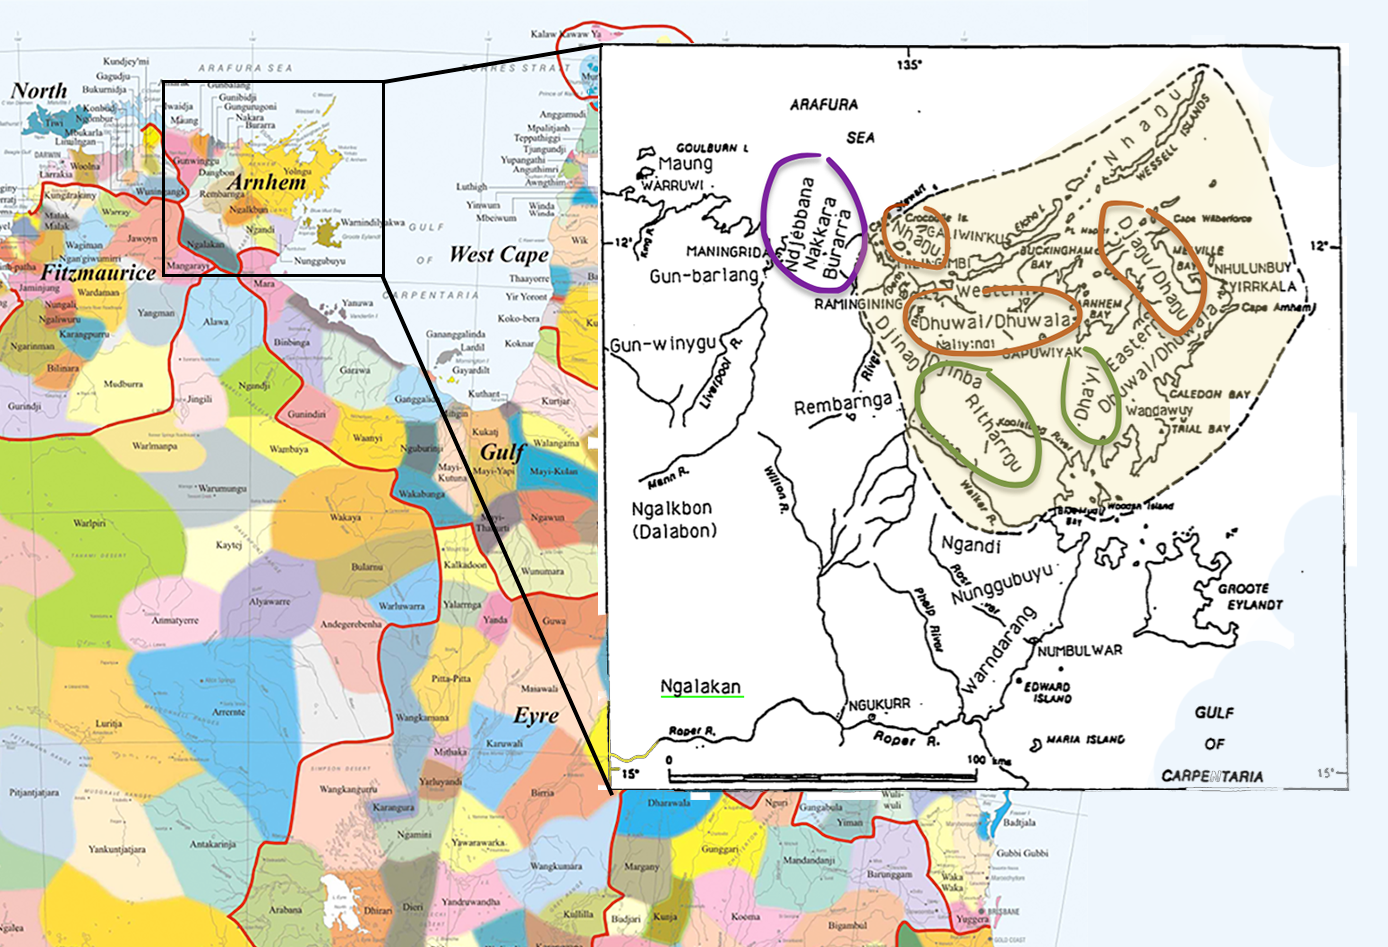
\includegraphics[width=0.7\textwidth]{AustralianLangsCropped.png}\label{map}
\end{figure}




%\section{Dhuwal-Dhuwala: Djambarrpuyŋu \& Gupapuyŋu}\label{djr}

TMA distinctions in Dhuwal(a) are encoded in a paradigm that disinguishes four `inflections', which are cognate with a number proto-Yolŋu inflections according to the reconstructions provided by \citet{Bowern2009}. Work on Dhuwal and Dhuwala varieties (notably \citealt{Wilkinson1991,Lowe1996}) has eschewed a metalinguistic gloss for these inflections, given the ostensible non-unifiability of their semantics. Both authors appeal to an arbitrary numbering system for the four ``inflections'', which I follow in this section. In addition to these inflections, the expressive burden of encoding TMA relations is shared by a (closed) class of auxiliaries, which appear to interact with the verbal paradigm. 

Further complicating the exposition of this, is the fact that there are a number of \textit{conjugation (sub)classes}: 9 according to \citet{Lowe1996} for Gupapuyŋu, 3 larger classes each with a number of subclasses in addition to ``non-inflecting'' and (semi-)irregular categories for the closer description in \citet{Wilkinson1991}.

In this section, I draw predominantly from existing and novel resources on the Djambarrpuyŋu (comprehensively documented by Melanie Wilkinson \citeyearpar{Wilkinson1991}) and Gupapuyŋu (especially with reference to Beulah Lowe's grammar notes and Anita van der Wal's \citeyear{VanderWal1992} doctoralthesis). These two central Arnhem varieties are closely related. Additional references are made to the eastern varieties Djapu \citep{Heath1980b,Morphy1983} and Gumatj. Wilkinson's proposed  phylogeny of Southern Yolŋu is provided (slightly simplified \& modified) as Figure \ref{DDvars} below. See Chapter \ref{ecology} for more background.

\begin{figure}[h]\centering
\begin{tikzpicture}[every node/.append style={align=left},every tree node/.style={anchor=north}]
\Tree [.\textsc{\textbf{Southern~Yolŋu}} [.\textbf{Ritharrŋu} $\vdots$ ] [ [.\textbf{Dhay'yi} $\vdots$ ] [.\textbf{Dhuwal-Dhuwala} [.\textsc{western} \node[text=teal,font=\itshape]{\bf\it Djambarrpuyŋu\\Ḻiyagalawumirr\\Ḻiyagawumirr\\Marraŋu}; \node[font=\itshape,text=ochre]{\bf\it Gupapuyŋu\\Wubulkarra}; ]   [.\textsc{eastern} \node[font=\itshape,text=teal] {Djapu\\Marrakulu\\Ḏäṯiwuy}; \node[font=\itshape,text=ochre]{Gumatj\\Maŋgalili\\Munyuku\\Maḏarrpa}; ] ] ] ]
\end{tikzpicture}
\caption{Varieties (dialects) of \textcolor{teal}{Dhuwal}-\textcolor{ochre}{Dhuwala} in the context of the Southern Yolŋu languages \citep[following][13]{Wilkinson1991}.}\label{DDvars}
\end{figure}

\section{The verbal inflections \& their functional domains}\label{infls}

As mentioned above, Dhuwal(a) varieties make use of a verbal paradigm with four inflectional distinctions. As discussed in Chapter \ref{ecology}, varieties of Dhuwal-Dhuwala are mutually intelligible, the primary distinction resulting from a productive apocope rule (\citealp[51]{Morphy1977}, \citealp[see also][94\textit{ff}]{Wilkinson1991} for further details.). The formal consequences of Dhuwal apocope on the verbal paradigm are shown in Table \ref{djr-pdm-exx} below. The table gives examples of the verb paradigm for each of the major Djambarrpuyŋu conjugation classes as described by \citet[306ff]{Wilkinson1991} (parentheses give the corresponding verb group number assigned by \citet{Lowe1996} for Gupapuyŋu.)

\mcom{Of course I can provide more detailed information (the subclasses) but that feels like it'd be better appended? The comparative spreadsheet i've made/Claire's 2009 stuff has most of this formative data... \\\textbf{note: Andrea Simms strongly suggests more exposition of the formal paradigm} }\begin{table}[h]\centering
	\begin{tabular}{ll|llll}
		\textbf{Class} & \textbf{\textit{Example}} & \textbf{I} & \textbf{II} & \textbf{III} & \textbf{IV}\\\midrule
		$\boldsymbol\emptyset$  (2)& \textit{marrtji} `go' & \textit{marrtji}& \textit{marrtji} & \textit{marrtji\textbf{n(a)}} & \textit{marrtji\textbf{nya}}\\
		
		$\boldsymbol\emptyset_{rr}$  (?)& \textit{waṉḏirr(i)} `run' & \textit{waṉḏi\textbf{rr(i)}}& \textit{waṉḏi} & \textit{waṉḏi\textbf{n(a)}} & \textit{waṉḏi\textbf{nya}}\\
		
		
		
		\textbf{N} (5) & \textit{ḻupthun} `wash' &\textit{ḻuphtu\textbf{n}} & \textit{ḻupthu\textbf{rr(u)}} & \textit{ḻupthu\textbf{rr(una)}} & \textit{ḻupthu\textbf{na}}\\
		 \textbf{Ŋ} (7)  & \textit{nhäma} `see' & \textit{nhä\textbf{ma}} & \textit{nhä\textbf{ŋu}} & \textit{nhä\textbf{ŋal(a)}} & \textit{nhä\textbf{nha}}\\
				\end{tabular}
			\caption{Examples of the paradigm of four morphological TMA inflections in Djambarrpuyŋu [\gls{djr}] and (Gupapuyŋu [\gls{guf}] resyllabification in parentheses).\\{}[\gls{djr}] data from \citet{Wilkinson1991}; [\gls{guf}] data from \textit{Gupapuyŋu} \citeyearpar{Gupapuyngu2016}.} \label{djr-pdm-exx}
\end{table}

In the first paragraph of this section, I alluded to Beulah Lowe's eschewal of a ``semantic description'' for each of the four inflectional classes. Melanie Wilkinson follows this system in her 1991 grammar and I will follow them here. Below I provide examples of the functional domains of each of the four inflections in Dhuwal-Dhuwala. Inflections are glossed with the bold-faced Roman numerals given in Table \ref{djr-pdm-exx}. This section focuses on the interpretation received by inflections in simple sentences (\textit{sc.} matrix clauses) -- complex sentences and predications are investigated in further detail in §\ref{djr-subord}.

Table \ref{Infl-Comparisons-Wilk}, adapted from \citet[336]{Wilkinson1991} summarises the metalanguage decisions made by other authors in their attempts to describe Dhuwal(a) varieties.

\begin{table}[h]
\begin{tabular}{l|llll}
	&	\textbf{I}	& \textbf{II}	&	\textbf{III}	&	\textbf{IV}\\\midrule
\citealt{Wilkinson1991} (Djambarrpuyŋu)&\textsc{First}&\textsc{Second}&\textsc{Third}&\textsc{Fourth}\\
\citealt{Lowe1996} (Gupapuyŋu) &Primary&Secondary&Tertiary&Quartenary\\
\citealt{Tchekhoff1983} (Djambarrpuyŋu)&\textsc{Bas}e&\textsc{Fut}ure&Past\textsubscript1&Past\textsubscript2\\
\citealt{Heath1980} (Dhuwal) & Pres/Fut & Fut/Imp & Past & Past Remote\\
\citealt{Morphy1983} (Djapu) & Unmarked & Potential & Perfective & Past Non-indicative\\
\end{tabular}
\caption{Summary of metalinguistic descriptors for the four inflectional classes in a number of Dhuwal/Dhuwala varities, adapted from \citet[336]{Wilkinson1991}.}\label{Infl-Comparisons-Wilk}
\end{table}

\subsection{The Primary inflection}

The `primary' inflection (\textbf{I}), cognate with inflections in other Yolŋu languages which have been described as ``unmarked'' or ``base'', surfaces in predications about the present, past and future. Here I provide examples of \textbf{I}-inflected clauses receiving each of these temporal interpretations.

\mcom{Now for both of these (and i suspect all sentences in this sssection) context ought to be modulable s.t. a non-present reading is available. This can/should/will be tested in the field}\pex\textit{ Present-reference encoded with \textbf{I}}

\a\begingl\deftagex{IPres}\deftaglabel{nhina}
\gla Ŋunhi-y ŋunhi ḏirramu \textbf{nhina} ga//
\glb \gls{texd}\textsc{-erg} \textsc{texd} man sit.\textbf{I} \textsc{ipfv.\textbf{I}}//
\glft`There that man is sitting.'\trailingcitation{\citep[856]{Tchekhoff1983}}// 
\endgl
%\a\begingl \gla ŋarra \textbf{marrtji}-n dhiyaŋu-n bala//
%\glb 1s go\textbf{.I}-\gls{seq} \gls{prox}.\gls{erg}-\textsc{seq} then//
%\glft`I am going now.'\trailingcitation{\citep[256]{Wilkinson1991}}//\endgl
\a\begingl\gla Ŋarra ga \textbf{ḻuka} gapu (dhiyaŋu bala)//
\glb 1s \textsc{ipfv.\textbf{I}} consume.\textbf{I} water \gls{texd}.\gls{erg} then//
\glft`I'm drinking water at the moment.'\trailingcitation{[DhG 20190405]}//\endgl
\xe

The sentences given in (\getref{IPres}) show the compatibility between present temporal reference and the \textbf{I} inflection: in both cases, the event described by the predicate (\textit{nhina} `sit.\textbf{I}' and \textit{marrtji} `go.\textbf{I}') is understood as being contemporaneous with speech time. Both sentences receive event-in-progress readings (also co-occurring with explicit aspectual marking, see §\ref{djr-asp} for more.)

\mcom{Is it a shitty idea to use colour coding for more formatting/highlighting options? I want to resolve bold for the verbforms themselves but would like to be able to second-order emphasise non-paradigmatic things like TFAs, aspectual ops...}
\pex \textit{Past-reference encoded with \textbf{I}}\deftagex{pstI}

%\a\deftaglabel{nhama}\begingl\gla barpuru linyu \textbf{nhäma} dirramu-ny//
%\glb yesterday 2d see.\textbf{I} boy-\gls{acc}//
%\glft`Yesterday we saw a boy'\trailingcitation{\citep[569]{Tchekhoff1985}}//\endgl


\a\deftaglabel{ŋayatham}\begingl\gla ga \textbf{ŋayatham} ŋunha baṉ'thula-wuy ŋayambalk//
\glb and reach.\textbf{I} \gls{dist} \textsc{place}-\gls{assoc} place//
\glft`And (then we) reached the place (associated with) Baṉthula.'\trailingcitation{\citep[461]{Wilkinson1991}}//\endgl



\a\deftaglabel{rrupiya}\begingl\gla ḏirramu-wal yothu-wal bäpa-'mirriŋu-y rrupiya barpuru djuy'yu-\textbf{n} märr barpuru ga barpuru \textbf{buna}-ny dhiyal-nydja//
\glb man-\gls{obl} kid-\gls{obl} father-\gls{kinprop}-\textsc{erg} money yesterday send.\textbf{I} somewhat yesterday and yesterday arrive.\textbf{I}-\textsc{prom} \gls{prox}.\gls{erg}-\gls{prom}//
\glft`The father sent money to the boy recently and it arrived here yesterday'\trailingcitation{\citep[343]{Wilkinson1991}}//\endgl

\xe

Additionally, the sentences given in (\getfullref{pstI}) show compatibility between \textbf{I} and past time reference. For both examples the events described by the predicates (e.g. the seeing event described by \textit{nhäma} in (\getref{pstI.ŋayatham})) \textit{precede} speech time. Similarly, the two past events in (\getref{pstI.rrupiya}) both receive \textbf{I} inflection. The instantiation times of both of these events are restricted by with \textit{barpuru} $\approx$ `yesterday. -- frame adverbials of this type are discussed in some detail in §\ref{TFA}.

\pex \deftagex{futI} \textit{Future-reference encoded with \textbf{I}}
\a\deftaglabel{lakaram}\begingl\gla yalala ŋarra dhu nhokal lakara-\textbf{m}//
\glb later 1s \textsc{fut} 2s\textsc{.obl} tell-\textbf{I}//
\glft `Later (today) I'll tell you.' \trailingcitation{\citep[373]{Wilkinson1991}}//\endgl

\a\deftaglabel{buna}\begingl \gla dhiyaŋ~bala walal dhu \textbf{buna}, yalala//
\glb now 3p \textsc{fut} arrive.\textbf{I} later//
\glft`They are coming later today.'\trailingcitation{\citep[256]{Wilkinson1991}}//\endgl


\a\begingl\glpreamble Deontic force with \textit{dhu}+\textbf{I} (see §\ref{dhu})//
\gla Way! Nhe dhu gurruka-\textbf{m} helmet! Rom ga \textbf{waŋa}.//
\glb Hey! 2s \gls{fut} wear-\textbf{I} \textit{helmet} law \textsc{ipfv.\textbf{I}}  say.\textbf{I}//
\glft`Oy! You wear a helmet! The law says so!\trailingcitation{[AW~20170730]}//\endgl

\a\deftaglabel{marrtji}\mcom{Actually, W claims this is ``imminent action'' so we really just have a futurate use of \textbf{I} without \textit{dhu} (interesting data point in itself) This can probably move to the section on future marking (either \textbf{I} or \textbf{\textit{dhu}})}\begingl\glpreamble `Imminent action' without \textit{dhu}//
\gla \ljudge{$ ^{\%*} $}ŋarra marrtji-n \textbf{dhiyaŋu}-n \textbf{bala}//
\glb 1s go-\gls{seq} \textbf{\gls{prox}.\gls{erg}}-\gls{seq} \textbf{\gls{mvtawy}}//
\glft`I'm going now.'\trailingcitation{\citep[256]{Wilkinson1991}}//\endgl

\xe


Finally, the examples in (\getref{futI}) above, show the compatibility of \textbf{I}-inflected verb forms and future temporal reference. In both sentences, the event described by the predicate is understood to obtain in the \underline{future} of speech time (modulo additional constraints on imminence/immediacy described below). \mcom{Evidence of infelicity of \textit{dhu}-less future readings? I actually kinda doubt on the basis of Tonnhauser, Bohnemeyer's work that this is going to be a hard constraint} In these sentences the presence of \textsc{fut} marker \textit{dhu} is apparently obligatory in order to establish future reference. (Although according to \citet[256]{Wilkinson1991} (\getfullref{futI.marrtji}), a futurate interpretation is ostensibly available. This use is unavailable to Ramingining speakers.

\subsection{The Secondary inflection}

Like \textbf{I}, the Secondary inflection (\textbf{II}) has a range of uses. It is notably obligatory when predicating of future times \underline{beyond the current day} and is the main strategy for forming \underline{imperative sentences}.

\pex\deftagex{futII} \textit{Future-reference encoded with \textbf{II}}
\a\deftaglabel{lakaraŋ}\begingl\glpreamble Co-occurring with \textit{dhu} `\gls{fut}'//
\gla yalala-ŋu-mirri-y ŋula~nhätha ŋarra dhu nhokal lakara\textbf{-ŋ}//
\glb later-\textit{ŋu}-\gls{prop}-\gls{erg} sometime 1s \textsc{fut} 2s-\gls{obl} tell-\textbf{II}//
\glft`I'll tell you sometime later on'\trailingcitation{\citep[346]{Wilkinson1991}}//
\endgl
\a\deftaglabel{nhini}\begingl\glpreamble Future interpretation independent of \textit{dhu} `\gls{fut}'//
\gla ŋayi boŋguŋ \textbf{nhini} \textbf{ŋäku} ŋarra-ny ŋunhal yirrkala//
\glb 3s tomorrow sit.\textbf{II} hear.\textbf{II} 1s-\gls{prom} \gls{dist}-\gls{loc} \textsc{placename}//
\glft`She'll be there at Yirrkala tomorrow, listening to me'\trailingcitation{\citep[340]{Wilkinson1991}}//\endgl

\a\begingl\glpreamble Infelicity of \textbf{I} with non-today future//
\gla Barpuru goḏarr ŋarra dhu nhä(\textbf{-ŋu/$^*$-ma})//
\glb funeral tomorrow 1s \gls{fut} see(-\textbf{II}/$^*$-\textbf{I})//
\glft `I'll see the funeral tomorrow'\trailingcitation{[AW~20180730]}//\endgl

\xe

The two sentences in (\getref{futII}) show how \textbf{II} is used to establish future temporal reference. The conditions on the (non-)appearance of \textsc{fut}-marker \textit{dhu} are unclear at the present time (see §\ref{dhu} for more), but future-readings with \textbf{II} do not appear to be reliant on this auxiliary (cf. the data in (\getref{futI}) above). A notable contrast between (\getfullref{futI.lakaram}) and (\getfullref{futII.lakaraŋ}) is the apparently obligatory retrieval of a \textsc{today}-reference time for \textbf{I}-inflected futures, as against a (probable) \textsc{beyond-today}-reference time for \textbf{II}-inflected futures.\footnote{\citet[347]{Wilkinson1991} gives an example of a speaker using a \textit{dhu}-\textbf{II} structure in the context of a narrative she is telling, signalling that she `will (return to the time of the old people).' Wilkinson takes this as evidence of an association between \textbf{II} and the irrealis. This generalisation is pursued in detail in the next chapter of this dissertation.} Effectively, this distinction seems to be one place where the grammar of Dhuwal(a) grammaticalises ``temporal remoteness'' (\citet{Comrie1985,Dahl1985} referred to elsewhere in the literature as `metrical tense' \citealp[e.g.][204]{Chung}).\footnote{Although \citet[39]{Heath1980} suggests of the \textbf{II} future in Dhuwal Proper (his \textsc{Fut/Imp}) that this form encodes a type of ``normative nuance'' (a clear extention of imperative flavour into future assertions.)}


\mcom{It would be good to get sentences with richer context (i.e. an established time of instantiation for the prejacent (tomorrow, imminently etc...)) This said we can probably assume that the we're talking about immediate future here... Is \textbf{I} incompatible with this? There's not much more to say here until I have speaker judgments on this question.}\pex\deftagex{irrII}\begingl\gla Ŋarra ŋuli bäynha \textbf{dhiŋgun} ŋawulul-yu//
\glb 1s \textsc{hyp?} \textsc{mod?} die.\textbf{II?} smoke-\textsc{erg?}//
\glft`I might die from the smoke.'\trailingcitation{\citep[164]{Buchanan1978}}//\endgl\xe


(\getref{irrII}) shows the compatibility of \textbf{II} with a future-oriented possibility reading. The modal particles \textit{ŋuli} and \textit{bäynha} are responsible for the `weakening' or `downtowning' of the speaker's commitment to the prejacent proposition. Modal operators are described in §\ref{modals}.


\pex\textit{Imperative force with \textbf{II}}\deftagex{impII}
%\a\begingl\gla g...y, ḻupmara-\textbf{ŋu}-n ŋarra-ny//
%\glb \textsc{name} wash-\textbf{II}-\gls{seq} 1s-\gls{prom}//
%\glft`G...y, wash me!'\trailingcitation{\citep[360]{Wilkinson1991}}//\endgl

\a\begingl\gla wäy! gurtha ŋunha, nhawi, ḏutji män-\textbf{ŋu}, bakmara-\textbf{ŋu}//
\glb hey! fire(wood) \gls{dist} what's.it firesticks get-\textbf{II} break\textbf{-II}//
\glft`Hey! Get that firewood, what's it, those firesticks, and break them.'\trailingcitation{\cite[114]{VanderWal1992}}//\endgl




\a\deftaglabel{proh}\begingl\gla yaka walala-ŋ buku-bakamara-\textbf{ŋ}//
\glb \gls{neg} 3p-\gls{dat} head-break-\textbf{II}//
\glft `Don't answer them!'\trailingcitation{\citep[360]{Wilkinson1991}}//\endgl


\a\begingl\gla nhä\textbf{-ŋu} nhanŋu dhurrwara!//
\glb look-\textbf{II} 2s.\gls{dat} door//
\glft`Look at her mouth!'\trailingcitation[AW 20180731]//\endgl

\xe


The sentences in (\getref{impII}) show the imperative function of \textbf{II}-inflected clauses. Shown in (\getfullref{impII.proh}), negative imperatives (probibitives) are treated identically.\footnote{Although the use of privative-marked nominals is another common strategy, se.e \citet{Phillips2018a,Phillips2019} for more.}

\subsection{The Tertiary inflection}

The Tertiary inflection (\textbf{III}) is generally associated with predications about the \textsc{past}. An important caveat, however, is that this inflection is \ul{infelicitous when describing \textsc{recent} events instantiated \textsc{before the current day}.} The examples in (\nextx) below show the compatibility between \textbf{III} and a reference time that is `earlier today.'\mcom{Show the compatibility of \textbf{III} with \gls{ipfv} by adding some examples with \textit{gana}. (Perhaps a minimal pair, though this might be better placed below.)}

\pex \textit{\textsc{Today past} and the \textbf{III} inflection}\deftagex{pstIII}
\a\deftaglabel{gathur}\begingl\gla Gäthur ŋayi \textbf{marrtjin} räli Galiwin'ku-ŋur//
\glb today 3s go.\textbf{III} hither \textsc{place}-\gls{abl}//
\glft`[Earlier] today he came from Galiwin'ku.'\trailingcitation{\citep[150]{Buchanan1978}}//\endgl

\a\deftaglabel{bili}\begingl\gla Bili ŋayi \textbf{marrtjin} dhipuŋur natha-ŋur nyan'thuna-ŋur//
\glb \textsc{compl} 3s go.\textbf{III} \textsc{prox.abl} food-\gls{abl} eat.\textbf{IV}-\textsc{abl}//
\glft`He has already gone from having lunch here.'\trailingcitation{\citep[150]{Buchanan1978}}//\endgl


\a\begingl\glpreamble Infelicity of \textbf{III} with \textsc{recent past}//
\gla barpuru ŋarra nhä\textbf{(-ma/*-ŋala)} ḏetuŋ//
\glb yesterday 1s see\textbf{(-I/$^\#$-III)} buffalo//
\glft`I saw a buffalo yesterday.'\trailingcitation[MD 20180802]//\endgl

\a\begingl\glpreamble Infelctity of \textbf{I} with \textsc{today past}//
\gla gathura ŋarra nhä\textbf{($^\#$-ma/-ŋala)} ḏetuŋ dhukarra-ŋura//
\glb today 1s see\textbf{$ ^\# $-I/III} buffalo road-\gls{loc}//
\glft `I saw a buffalo today'\trailingcitation{[MD 20180802]}\\\textsc{comment.} Event could have happened this morning or ten minutes before speech time.//\endgl
\xe

\mcom{Potentially look for a ref for this or provide data that makes this unambiguous...}(\getfullref{pstIII.gathur}) shows the compatibility between temporal frame adverbial (TFA) \textit{gäthur(a)} `today' and \textbf{III} in \gls{djr}, which leads to an temporal interpretation of `earlier today.'\footnote{Note however that the reckoning of \gls{tfa} \textit{gäthur(a)} differs to that of English and other familiar languages as shown in (\getfullref{neg-pst.munha}), where \textit{gäthur munhawa} `today nighttime' is interpreted as ``last night'' and still triggers \textbf{III} marking on the verb.} However even in the absence of a \gls{TFA}, the event described in (\getref{pstIII.bili}) is interpreted as having been instantiated \textsc{earlier.today}/in the immediate past of speech time. \textbf{III} cannot, however, be conveniently described as a `hodiernal past' (cf. Mwera?, also \citealt[86]{Comrie1985}), as the data in (\nextx) make clear.


\pex\textit{\textsc{Remote past} and the \textbf{III} inflection}\deftagex{remIII}

\a\deftaglabel{wawa}\begingl\gla nhä nho-kiyin-gal wäwa-'mirriŋu-y warkthu-rr ŋäthil rarrandharr-yu//
\glb what 2s-\textsc{emph}-\gls{obl} bro-\gls{kinprop}-\gls{erg} work-\textbf{III} before dry~season-\gls{erg}//
\glft`What did your brother do last summer?'\trailingcitation{\citep[343]{Wilkinson1991}}//\endgl

\a\deftaglabel{malwan}\begingl\glpreamble\textsc{context.} The speaker is describing a locality as it was in her youth.//
\gla märrma' ga-\textbf{n} malwan-dja dhärra-\textbf{n} yindi maṉḍa-ny//
\glb two \textsc{ipfv}-\textbf{III} hibiscus-\gls{prom} stand-\textbf{III} big 3d-\gls{prom}//
\glft`Two big hibiscus flowers were (growing).'\trailingcitation{\citep[339]{Wilkinson1991}}//\endgl

\a\deftaglabel{wuŋgan}\begingl\glpreamble\textsc{context.} A man is telling a story from long ago . His friend's dog has spotted a water goanna.//
\gla ...ŋunhi wurkaḏi-y nhä-ŋal-{na} ŋinya dharpa-lil-a ŋal'yu-na nhäwi wan'kawu-ya//
\glb \gls{texd} \textsc{name}-\gls{erg} see-\textbf{III} 3s.\gls{acc} tree-\gls{all}-\gls{seq} ascend-\textbf{III} whatsit water.goanna-\gls{ana}//
\glft`\textit{Wukaḏi} watched it scramble up into a tree, the water goanna.'\trailingcitation{\citep[193]{Heath1980b}}//\endgl\mcom{I've taken some liberties with the glossing here, Heath has the second verb \textit{ŋal'yuna} as \textbf{I} with a \textsc{seq} marker... to investigate further perhaps}



\xe


Unlike the \textsc{hodiernal} temporal interpretations that the sentences in (\blastx) receive, the two sentences in (\lastx) are evaluated to obtain in the `\textsc{remote past}.' In (\getfullref{remIII.wawa}),\mcom{may be easier just to get a similar non-interrogative sentence to do what \lastx b does} the instantiation time of the predicate is restricted by two frame adverbials: \textit{ŋäthil(i)}, which picks out a time `in the distant past; prior to/earlier than (some other predicate)' \citep[158]{Wilkinson1991} and \textit{rarrandharryu} `dry season':\footnote{The suffix \textit{-Thu} (\textit{-yu} as a postsonorant allomorph), glossed here as \gls{erg} is used to mark ergative NPs as well as instrumental (\gls{instr}) NPs and to form TFAs out of nominals \gls{temp}.} The cooccurrence of these expressions restricts the predicate being questioned to \textit{a prior dry season}. Conversely, the declarative sentence in (\getfullref{remIII.malwan}) requires no adverbial specification. A \textsc{remote past} interpretation arises as a result of the \textbf{III} inflection alone, which is precised pragmatically by the discourse context (\textit{sc.} a narrative that the speaker is telling about her childhood.)\mcom{Provide some negative felicity judgments} In principle, \getfullref{remIII.malwan} ought to be able to retrieve a same-day past interpretation as well, with sufficient contextual support.

\mcom{This discussion of the Maningrida treatments of `frame' and `tense' may be better placed • entirely in the lit. review, • after the general data discussion of inflections, or • in the following chapter.} The ostensible `discontinuity' of the times predicates receiving \textbf{I} and \textbf{III} inflection can refer to has been described in preceding literature as \textbf{\textsc{cyclic time reference}} \citep[88]{Comrie1983}. In her influential treatment of Burarra [\gls{bvr}], \citet{Glasgow1964} draws a distinction between `tense' and `frame of reference' (`timescale' for \citealt[48]{Green1987}). The interaction between these is taken to give rise to a reference interval. This analysis has been adopted and developed by others working on Maningrida languages (\citet[165]{Eather2011} for Nakkara [\gls{nck}], \citet{Green1995} for Gurr-goni [\gls{gge}] and \citet{McKay2000}.) This is schematised in Table \ref{GlaswegianTR}. The following chapter further treats and formalises this analysis.


% Please add the following required packages to your document preamble:
% \usepackage{booktabs}
% \usepackage{multirow}
\begin{table}[h]\centering\onehalfspacing
	\begin{tabular}{@{}llll@{}}\toprule

		&                 & \multicolumn{2}{c}{\textsc{frame}}          \\ 
		&                 & \multicolumn{1}{c}{\textbf{today}}         & \multicolumn{1}{c}{\textbf{before today}}      \\\midrule
		\multirow{2}{*}{\textsc{\rotatebox[origin=c]{90}{infl}}} & \textbf{\phantom{I}I}    & now           & yesterday/recently \\
		& \textbf{III} & earlier today & long ago           \\ \bottomrule%(l){2-4} 
	\end{tabular}
\caption{A \citet{Glasgow1964}-style analysis of \textbf{past-time restrictions} introduced by the verbal inflections, adapted for the Dhuwal(a) data. \textbf{I} and \textbf{III} inflections correspond to Eather's \textbf{contemporary} and \textbf{precontemporary} ``tenses'' (``precontemporary'' is Eather's \citeyearpar[166]{Eather2011} relabelling of Glasgow's ``remote'' tense.)}\label{GlaswegianTR}
\end{table}
\mcom{Also the get sick/psych/phys condition verbs, some examples also in Buchanan:168}


Additionally, a set of psychological predicates that are frequently translated into English as present-tensed stative verbs appear with \textbf{III}. Examples are given in (\nextx).


\pex\deftagex{psychPreds}\a\begingl\gla ŋarra dhuwal/dhika djawaryu-\textbf{rr}/rerrikthu-\textbf{rr}/djanŋarrthi-\textbf{n}//
\glb 1s \textsc{prox/indefp} be.tired-\textbf{III}/be.sick-\textbf{III}/be.hungry-\textbf{III}//
\glft`I'm (a bit) tired/sick/hungry'\trailingcitation{\citep[278]{Wilkinson1991}}//\endgl
\a\begingl\gla bili djawar'yu-\textbf{rr}-a//
\glb \gls{cplv} be.tired-\textbf{III}//
\glft`They're already tired'\trailingcitation{\citep[365]{Wilkinson1991}}//\endgl
\mcom{Needs elicitation work, appears to be a today-past thing? Are these predicates available with TFAs \textit{barpuru?}, with \textit{ga}? And the other inflections??\\
Test entailments also: \textit{??I was tired this morning but i'm not now??}}
\a\deftaglabel{nhaŋal}\begingl\gla ŋarra dhu dhuwal lakara-m ƞunhi nhä ŋarra nhä-\textbf{ŋal} dhiyaŋ bala//
\glb 1s \gls{fut} \gls{prox} tell-\textbf{I} \gls{texd} what 1s see-\textbf{III} \gls{prox}.\gls{erg} \gls{mvtawy}//
\glft`I'll tell you what I see right now.'\trailingcitation{\citep{Wilkinson1991}}//\endgl
\xe

\citet[365-6]{Wilkinson1991}, in effect, suggests that the frequent exponence of \textbf{III} in these predicates of ``emotional and bodily states'' is a function of their lexical semantics. Unlike their English translations, with \textbf{III}, these predicates can be understood as `achievements' (to borrow from Vendler's Aktionsart taxonomy). In these cases then, \textbf{III} is licensed because \textit{djarwaryu\textbf{rr(u)}} refers to a state-change before speech time. Consequently, the licensing of \textbf{III} in (\getfullref{psychPreds.nhaŋal}) above is a consequence of a completed \textit{seeing} eventuality immediately prior to the \textit{telling}-event described in the matrix clause. This phenomenon is investigated in detail in §\ref{anY}\texttt{.1?} below.


\subsection{The Quaternary inflection}


\mcom{Is this XLinguistic note worth anything? If so a couple more examples would be nice.}The Quartenary inflection (\textbf{IV}) has a broad range of uses in Dhuwal(a) varieties that correspond in part to categories described in Australian languages including \textit{past potentialis} \citep{Heath1980a}, \textit{past counterfactual} \cite{McKay2011}, \textit{[past] irrealis} \citep[159]{Austin1998} \textit{etc.} It is used primarily with modal auxiliaries in order to describe past habituals (\getref{habIV}) with \textit{ŋuli} and past irrealis event description (with \textit{balaŋ} a.o.) as in (\getref{hypIV}) including counterfactuals.


\pex\a\deftagex{habIV}\begingl\gla Ŋayi ŋuli märra-\textbf{nha} ŋunhi meṉḏuŋ-nha//
\glb 3s \gls{hab} get-\textbf{IV} \gls{texd} snail-\gls{acc}//
\glft`She would (used to) get (collect) snails'\trailingcitation{\citep[147]{Buchanan1978}}//\endgl

\mcom{check ft for (b)}\a\begingl\gla ...ŋorra-\textbf{nha} walal ŋuli marrtji-\textbf{nya} ŋunhi-li-yi, galku-\textbf{na} walal ŋuli ga-\textbf{nha} gapuw wirwiryu-\textbf{na}+ra-w//
\glb lie-\textbf{IV} 3p \textsc{hab} go-\textbf{IV} \textsc{texd}-\gls{loc}-\gls{ana} wait-\textbf{IV} 3p \textsc{hab} \textsc{ipfv}-\textbf{IV} water-\gls{dat} turn-\gls{nmlzr}-\gls{dat}//
\glft`They would be lying there, they would be waiting for the water to stir.'\trailingcitation{(DB Djon 5:4)}//\endgl

\xe


\pex\a\begingl\glpreamble\deftagex{hypIV}\textsc{context.} Speaker had a toothache.//
\gla barpuru balaŋ ŋarra bala dentist-kal marrtji-\textbf{nya} dhiyak//
\glb yesterday \textsc{irr} 1s \gls{mvtawy} dentist-\gls{obl} go-\textbf{IV} \gls{prox}-\gls{dat}//
\glft`Yesterday I should have gone to the dentist for a filling'\trailingcitation{\citep[353]{Wilkinson1991}}//\endgl

\a\begingl\gla Yaka balaŋ nhe marrtji-\textbf{nya} Darwin-lil//
\glb \gls{neg} \textsc{irr} 2s go.\textbf{IV} Darwin-\gls{all}//
\glft`You should not go to Darwin.'\trailingcitation{\citep[164]{Buchanan1978}}//\endgl\xe


These data demonstrate the relationship between the \textbf{IV} inflection and combinations of past temporal reference and various modal and aspectual operators. These categories are treated in more detail in §\ref{modals} below. Furthermore, the data presented so for in this section are predominantly positive sentences. §\ref{negs} describes striking interactions between negation operators and verbal inflectional categories in some Dhuwal(a) varieties.

\section{Sentential negation: \textit{yaka} \& \textit{bäyŋu}}\label{negs}

Djambarrpuyŋu has two negative particles, \textit{yaka} and \textit{bäyŋu}, which are deployed for standard negation (i.e. those particles whose effect is to reverse the truth value of a given proposition.) The particles differ in that only \textit{yaka} is used to generate negative imperatives (prohibitives) and only \textit{bäyŋu} is found in negative existential/quantificational contexts (see \citet{Phillips2019b} for further discussion of semantic change in the Yolŋu negative domain.) Remarkable, however, is the complex interaction between sentential negation and verbal inflection.

Descriptively, negation appears to trigger a ``switch'' from the `realis-aligned inflections' (\textbf{I}~and~\textbf{III}) to their `irrealis counterparts' (\textbf{II}~and~\textbf{IV}), effectively evincing a mood-based distinction that is neutralised in negated sentences \citep[following ][356]{Wilkinson1991}. This is schematised below in Table \ref{negneut}.

\begin{table}[h]\centering
	\begin{tabular}{ccc}
		&\multicolumn{2}{c}{\textsc{\textbf{polarity}}} \\
		& \textsc{--neg} & \textsc{+neg}\\\midrule
	&	\textbf{I} & \multirow{2}{*}{\textbf{II}}\\
	& \textbf{II} \\\midrule
	&	\textbf{III} & \multirow{2}{*}{\textbf{IV}}\\
	& \textbf{IV} \\\bottomrule
	\end{tabular}
\caption{Neutralisation of \textbf{I} and \textbf{III} inflections under negation.}\label{negneut}
\end{table}


\pex\textit{Present/recent.past \textbf{I} expones as \textbf{II} under negation}\label{neg-pres}


\a\begingl\glpreamble  Negated present-tense sentence receives \textbf{II} marking\\\textsc{context.} Speaker is trying to read from a computer screen.//
\gla bäyŋu ŋarra \textbf{gi} nhä-\textbf{ŋu}//
\glb \gls{negq} 1s \gls{ipfv}.\textbf{II} see-\textbf{II}//
\glft`I can't see (it).'\trailingcitation{[AW 2018030]}\\\textsc{comment.} \textit{nhäŋu} (`see.\textbf{II}') could also mean yesterday, in past.//\endgl

\a\begingl%\glpreamble Negated present-tense sentence receives \textbf{II} marking//
\gla yaka \textbf{gi} \textbf{biyak} rom waŋ-\textbf{i}//
\glb \gls{neg} \gls{ipfv}.\textbf{II} do.thusly.\textbf{II} law say-\textbf{II}//
\glft`That's not how the law is/what the law says.'\trailingcitation{\citep[357]{Wilkinson1991}}//\endgl


\a\begingl\glpreamble Present-tensed sentence with \textbf{I}//
\gla Nhaltja-\textbf{n} \textbf{ga} limurru-ŋgu-ny rom waŋ-\textbf{a}?//
\glb do.how-\textbf{I} \gls{ipfv}.\textbf{I} 1p.\gls{incl}-\gls{dat}-\gls{prom} law say-\textbf{I}//
\glft`What does our law say?'\trailingcitation{(DB~Luk~14.3)}//\endgl


\a\begingl\glpreamble Negated (recent) past-tensed sentence receives \textbf{II} marking.\\
\textsc{context.} A recent hunting trip, narrated in \textbf{I} for corresponding positive descriptions.//
\gla ga yaka ŋayi ŋunhi dharyu-rr biyak djin'tjiŋdhu-rr//
\glb and \gls{neg} 3s \gls{texd} rain-\textbf{II} do.thusly.\textbf{II} rain~lightly.\textbf{II}//
\glft`...and it did not rain lightly'\trailingcitation{\citep[357]{Wilkinson1991}}//
\endgl

\xe


\pex Past-tensed sentences exponing with \textbf{IV} under negation\deftagex{neg-pst}
\a\deftaglabel{munha}\begingl\gla bäyŋu ŋarra gäthur ŋorra-\textbf{nha} manymak-ku-\textbf{nha} munhawu//
\glb \gls{negq} 1s today lie-\textbf{IV} good-\gls{tr}-\textbf{IV} nighttime//
\glft`I didn't sleep well last ni	ght'\trailingcitation{\citep[357]{Wilkinson1991}}//\endgl

%\mcom{Though the second clause in (b) also has ŋuli so maybe this is not quite so nice an ex. as originally thought}\a\begingl\gla ŋäthil-nydja ŋarra ga-n dhuwal, ga miltjiri marrtji-n \ bäyŋu ŋarra ŋuli ga-\textbf{nha} nhä-\textbf{nha}//
%\glb earlier-\gls{prom} 1s \gls{ipfv}-\textbf{III} \gls{prox} and blind go-\textbf{III} \textbackslash \gls{negq} 1s \gls{hab} \gls{ipfv} see-\textbf{IV}//
%\glft`I was blind before; I was unable to see'\trailingcitation{\citep[358]{Wilkinson1991}}//\endgl


\a\begingl\gla gathur munhagumirr ŋarra nhä-\textbf{ŋal} warrakan//
\glb today morning 1s see-\textbf{III} bird//
\glft`I saw a bird this morning'\trailingcitation{[FW 20180802]}//\endgl


\a\begingl\gla gathur munhagumirr bäyŋu ŋarra nhä-\textbf{nha} warrakan//
\glb today morning \gls{neg} 1s see-\textbf{III} bird//
\glft`I didn't see a bird this morning'\trailingcitation{[FW 20180802]}//\endgl

\a\begingl\glpreamble \textsc{context.} Speaker has dropped a coin.//
\gla Way! Bäyŋu ŋarra nhä-nha?//
\glb Hey! \gls{negq} 1s see-\textbf{IV}//
\glft`Ah! Did you see (it)?'\trailingcitation{[AW 20180830]}//\endgl

\a\begingl\glpreamble Negated (distant) past receives \textbf{IV} marking.\\
\textsc{context.} The text describes remote past events, narrated in \textbf{III} for corresponding positive descriptions//
\gla ŋayi-ny muka bäyŋu yan yolŋu-ny yurrumdhu-\textbf{na}//
\glb 3s-\gls{prom} okay \gls{negq} \gls{emph}  person-\gls{prom} gather-\textbf{IV}//
\glft`Not all the people had gathered together'\trailingcitation{\citep[357]{Wilkinson1991}}//\endgl


\xe

\mcom{It's not clear how I can easily get a the status of this alternation via elicitation (esp. if its intraspeaker..?) or whether I should just abstract away from it. My informants so far seem to have consistently respected this alternation.}Notwithstanding this generalisation, \citet[358\textit{ff}]{Wilkinson1991} notes that there exists a considerable amount of synchronic variation in the formal (neutralising) relation between negation and inflection. \Citet[110]{VanderWal1992} in fact reports no asymmetry in her study of Gupapuyŋu, noting that it is just as valid to predict the affirmation of a proposition with future temporal reference as it is to predict the negation of such a proposition.' (\nextx) gives examples of `unexpected' realis-aligned inflections appearing under negation.

\pex Exponence of \textbf{I} and \textbf{III} under negation.


\a\begingl\gla ga yaka-na ŋarra yurru bulu roŋiyi-\textbf{rri}//
\glb and \gls{neg}-\gls{prom} 1s \gls{mod} again return-\textbf{I}//
\glft`And I will not come back again.'\trailingcitation{\citep[110]{VanderWal1992}}//
\endgl


\a\begingl \gla bäyŋu ŋayi ga dhuwal nhina dhiyaŋu-ny bala//
\glb \gls{negq} 3s \gls{ipfv}.\textbf{I} \gls{prox} sit.\textbf{I} \gls{prox}.\gls{dat}-\gls{prom} \gls{mvtawy}//
\glft`She isn't living here now'\trailingcitation{\citep[358]{Wilkinson1991}}//\endgl
\mcom{I suspect a good way of excluding this data will be to test its acceptability with my consultants. I expect Albert, Faith will reject all of these.\\If so is this whole discussion something that should be in fn or Ch.\ref{diaY} rather than in body here?}
\a\begingl \gla gurrupa-\textbf{r} muka ŋarra ga-\textbf{n}, yurr bäyŋu-n ŋayi ga-\textbf{n} ḻuka-\textbf{n}, ŋatha-ny//
\glb give-\textbf{III} \textsc{ok} 1s \gls{ipfv}-\textbf{III} but \gls{negq} 3s \gls{ipfv}-\textbf{III} eat-\textbf{III} food-\gls{prom}//
\glft`I was giving (him) the food but he wasn't eating it'\trailingcitation{\citep[358]{Wilkinson1991}}//\endgl

\xe

Generally, there seems to be a perception (Melanie Wilkinson \textit{pers. comm.}, independently supported by consultant AW [20180830]) that the maintenance of \textbf{I} and \textbf{III} (the `\textsc{realis}-aligned' inflections) under negation is a characteristic of \textit{Miwatj} varieties of Dhuwal-Dhuwala (i.e. those spoken in towards the East.) This is suggestive of an areal/contact phenomenon, a siutation to be further discussed in Chapter \ref{diaY}.

\mcom{There's a great comment from my consultant in her translation of a negative sentence. When asked why \textbf{\textit{gi+}II} was used instead of \textbf{\textit{ga+}I} she claims `not happening yet' (20180802-8min)}\citet[356]{Wilkinson1991} notes that ``[she has] not been able to determine a functional basis for this alternation.'' Nevertheless, in his typological survey of standard negation, \citet[558]{Miestamo2005} identifies a cross-linguistically attested mood-based asymmetry where negative marking triggers the appearance of the irrealis or other ``nonrealised''-type modal markings. This phenomenon seems to be particularly well-represented in the languages of the Top End, functional explanations generally emphasising the fact that negated predicates `[belong] to the realm of the non-realized', a domain associated with irrealis marking (\citealt[225]{Miestamo2005}, cf. \citealt[195]{McLellan1992}, \citealp[see also][]{Phillips2019}). These ideas are explored in further detail in Chapter \ref{anY} below.

\citet{Wilkinson1991} also suggests that there is insufficient cross-linguistic data to assess a the diachrony (and potential areal diffusion) of this asymmetry (356), although provides a concise review of other authors' observations of Yolŋu varieties (359-60). Data about the interactions between polarity and verbal inflection are provided in the following sections and the question of the development of these asymmetries is treated in Chapter \ref{diaY} below.


\section{\textit{dhu}}\label{dhu}

\textit{dhu} (and apparent synonym/dialectal variant \textit{yurru}) is treated as a \gls{fut}-particle by \citet[346]{Wilkinson1991}, Lowe and \citet[39,46]{Heath1980b}. Also available are deontic and epistemic modal readings (such that \citet[110]{VanderWal1992} glosses this particle as \gls{mod}.) These uses of \textit{dhu} are shown in (\getref{dhuT}-\getref{dhuM}) below.

\pex\deftagex{dhuT}\begingl\glpreamble Future reading of \textit{\textbf{dhu}}//
\gla yaka-na \textbf{dhu} limurru roŋiyi-\textbf{rri} Yirrkala-lili//
\glb \textsc{neg-foc} \textsc{\textbf{mod}} 1p\textsc{.inc} return-\textbf{I} Yirrkala\textsc{-all}//
\glft`We won't return to Yirrkala'\trailingcitation{\Citep[125]{VanderWal1992}}//\endgl\xe



\pex\deftagex{dhuM}\textit{Modal readings of \textbf{dhu}}




\a\begingl\glpreamble\textit{Deontic necessity reading of \textbf{dhu}}\\\textsc{context.} Speaker's 16 year-old \textit{waku} has just got his driver's license.//
\gla gaŋga nhe \textbf{dhu} ga gäma mutika-y//
\glb slowly 2s \textbf{\gls{fut}} \gls{ipfv} carry.\textbf{I} car-\gls{erg}//
\glft `You should/must drive slowly.'\trailingcitation{[FW?~20180802]}//\endgl
\mcom{elicit ''you should but you don't have to''\\A future deontic presumbaly takes \textbf{\textit{dhu}+II}}


\a\mcom{The ambiguity between circ nec and fut readings here is super interesting because it really throws the polysemy of \textit{bala} into relief as picking up either $ t* $ or $ w* $}\begingl\glpreamble \textit{Circumstantial necessity reading of \textbf{dhu}}\\\textsc{context.} Child drank a lot of water before boarding a now mid-flight aeroplane.//
\gla Bäpa, gupa ŋarra dhu (bala) waryu-n!//
\glb \textsc{Fa} water 1s \gls{fut} (\gls{mvtawy}) urinate-\textbf{I}//
\glft`Dad, I need to wee now!'\trailingcitation{[AW 20180830}//\endgl

\a\begingl\glpreamble \textit{Deontic impossibility reading of \textsc{neg+}\textbf{dhu}}//
\gla ga yaka-dhi walala \textbf{dhu} \textbf{ga} yatjun-\textbf{dhi}//
\glb and \textsc{neg-ana} 3p \textsc{\textbf{mod}} \textsc{cont.\textbf{I}} bad-\textbf{I}//
\glft`And they must not be disobedient'\trailingcitation{\Citep[125]{VanderWal1992}}//\endgl

\a\begingl\glpreamble\textit{Circumstantial impossibility reading of \textsc{neg}+\textbf{dhu}}\\\textsc{context.} \textit{Waku} has broken his leg and can't go dancing with his friends.//
\gla bäyŋu ŋarra \textbf{dhu} marrtji disco-lil... bili bäyŋu ŋarra gi marrtji//
\glb \gls{negq} 1s \textbf{\gls{fut}} go.\textbf{I|II} disco-\gls{all} because \gls{negq} 1s \gls{ipfv}.\textbf{II} go.\textbf{II}//
\glft`I can't go to the disco because I can't walk.'\trailingcitation{[FW?~20180802]}//\endgl

\xe 


\mcom{this makes sense from a functional perspective but i suspect heath's constraint is too strong and the Mel gets us what we need. Given the relative temporal unambiguity of \textbf{II}, it's probably just that explicit \textsc{fut}s are more helpful in \textbf{I} contexts.} Unlike the Djambarrpuyŋu data in (\getref{futII}) above that inspire Wilkinson's descption, \citet[39]{Heath1980b} claims that these particles do not co-occur with \textbf{II} in the Dhuwal varieties he describes.

\textit{Dhu} has an additional modal/aspectual component. Wilkinson claims that it is used in conjunction with \textbf{I} to describe `situations which pertain...to current lifestyles or activities... that hold in the present.'\footnote{Note the possibility of a felicitous translation of these sentences with \textit{will} in English as well.} An example of this use is given in (\nextx).

\pex\a\begingl\gla dharpa-y ŋayi \textbf{dhu} marrtji...//
\glb tree-\gls{erg} 3s \gls{fut} walk-\textbf{I}//
\glft`They walk with a stick...'//\endgl%\trailingcitation{\citep[411]{Wilkinson1991}}//\endgl

\a\begingl\gla dharpa-mirr napurr \textbf{dhu} lakara-m yolŋu-ny, ŋayi \textbf{dhu} ga marrtji bitja-n gä-nha-mi-rr//
\glb tree-\gls{prop} 1p.\gls{excl} \gls{fut} tell-\textbf{I} person-\gls{prom} 3s \gls{fut} \gls{ipfv}.\textbf{I} go.\textbf{I} do.thusly-\textbf{I} bear-\textbf{IV}-\gls{refl}-\textbf{I}//
\glft`We call a person ``stick-having'', who goes around bearing themself with a stick'\trailingcitation{\citep[411]{Wilkinson1991}} //\endgl\xe

\citet[346]{Wilkinson1991} suggests that this use of the \textsc{today future} (\textit{sc. dhu}+\textbf{I}) to describe potential contemporary specific situations', can be accommodated by extending the relevant ``time domain'' of \textbf{I} (i.e. ``today nonpast'') to \textbf{\textsc{nowadays}}. This notion is crucial to the analysis that I lay out in Chapter \ref{anY} below.

\mcom{The big question to answer in this sssection is what the actual status of \textit{dhu} is -- does it pick out an absolute future interval? or one relative to a higher $t$? Is it a prospective aspect marker? The Heath disagreement should be easy to deal with (if it's even the right characterisation.)}



\textcolor{violet}{I suspect that \textit{dhu} isn't an absolute future marker:}

\pex \begingl \gla Bala ŋayi marrtji-nya-mara-ŋala lakara-ŋal-nydja dhäwu-ny birrŋ'mara-ŋala [ŋunhi-ŋu-wuy-yi yothu-walaŋu-wuy-nydja] yolŋu'-yulŋu-wal-nydja bukmak-kal-nha, [ŋunhi walal ŋuli ga-nha gatjpu'yu-na ga dhukarr-nhäma ŋuriki-yi], ŋunhi \textbf{dhu} God-thu dhawaṯmarama-n ŋunhi-yi wäŋa-ny garrpi-na-mirri-ŋur-nydja rom-ŋur mala-ŋu-ŋur//
\glb then 3s go-\textbf{IV}-\gls{tr}-\textbf{III} tell-\textbf{III}-\gls{prom} story-\textsc{prom} spread-\textbf{III} [\gls{texd}-\textit{ŋu}-\textsc{obl}-\textsc{ana} child-\gls{obl}-\textsc{dat}-\textsc{prom}] people-\textsc{dat-prom} all-\textsc{dat-acc} [\textsc{texd} 3p \textsc{hab} \textsc{ipfv}-\textbf{IV} hope-\textbf{III?} \textsc{ipfv} road-see.\textbf{I} \textsc{texd.dat-assoc}] \textsc{texd} \textsc{\textbf{fut}} God-\textsc{erg} expel-\textbf{I?} \textsc{texd-ana} land-\textsc{prom} bind-\textbf{IV}=\gls{prop}-\gls{abl}-\gls{prom} law-\textsc{abl} group-\textit{ŋu}-\textsc{abl}//
\glft`Then she went about spreading the news [of that child] to all the people [that were hoping and looking out for it], that God would free the place from the laws that bound it'\trailingcitation{Godku dharuk p20}//\endgl\xe

\textcolor{violet}{\mcom{Other big question is how obligatory \textit{dhu} is in matrix clauses to get the future readings.} So \textit{dhu} in (\lastx) is picking out a time in the absolute past, but the future of a reference time established in the matrix clause. This suggests that \textit{dhu} relates event time (here the \textsc{free} predicate) and a ref (or top) time set by the embedding predicate. Note that it also seems to have coupled with a \textbf{I} inflection (although this isn't super clear.)}




\section{Aspectual auxiliaries}\label{djr-asp}

Overt aspectual marking is grammaticalised in a number of ways. This subsection is further divided; I discuss Djambarrpuyŋu grammatical strategies for marking the two major `inclusion' aspects -- the imperfective $\big(i\sqsubseteq \tau(e)\big)$ and perfective $\big(i\sqsupseteq \tau(e)\big)$ --- seperately below.

\subsection{Imperfectivity}\label{ipfvty}

 The most commonly occurring strategy for explicitly indicating imperfectivity is the auxiliary \textit{ga} `\gls{ipfv}', which ``agrees'' with the inflection of the verb that it modifies (\textit{i.e. } \textit{ga/gi/gan(a)/ganha}.) \citet[46]{Heath1980b} claims of the Dhuwal varieties he investigates that for \textbf{I}-inflected utterances, `\textit{[ga]} specifies present tense and \textit{[dhu]} specifies future tense.'\footnote{\citet[46]{Heath1980b} notes that [\textit{gan}] occurs ``usually with [\textbf{III} or \textbf{IV}] inflection, indicating durative'' but he makes no reference to compatibility of this auxiliary with future and does not go so far as give a completely aspectual analysis.} Given the close association between present-tensed utterances and imperfectivity (see \citealp[141]{Bybee1994},\texttt{ ref, ref, Deo}), there does seem to be a strong tendency for present-reference to associate with \textit{ga} as in (\getfullref{IPres.nhina}), although the presence of an imperfective auxiliary is neither a necessary nor sufficient condition for the emergence of present-readings.


\pex\begingl\gla yo, ŋarra yawungu ŋanya nhäma, ŋayi \textbf{ga} djäma ḏo'ŋur ŋunha Baṉ'thula//
\glb yes 1w yesterday 3s.\textsc{acc} see\textbf{.I} 3s \textsc{\textbf{ipfv}.I} work store \gls{dist} \textsc{place}//
\glft`Yes I saw him yesterday, he was working at the store in Baṉ'thula.'\trailingcitation{\citep[363]{Wilkinson1991}}//\endgl\xe


\citet[363-7]{Wilkinson1991} carefully shows the compatibility of \textit{ga} with all four inflectional categories and receiving past, present and future interpretations. I take this (parallel) distributional data as a clear demonstration that this auxiliary \ul{does not} directly encode tense.\footnote{In fact \citet[367]{Wilkinson1991} suggests that when a predicate receives past temporal reference (e.g. in the \textbf{I} and \textbf{III} inflections), a perfective reading is ``assumed'' in the absence of \textit{ga/gan}.}

Similarly, \textit{marrtji+\textsc{infl}} `go' alternates with auxiliary \textit{ga} `\textsc{ipfv'} \mcom{How would serialisation really be distinguished from auxiliarisation?}(perhaps in a variety of serial verb construction?) to encode another shade of imperfective meaning. \citet[369]{Wilkinson1991} suggests that this points to a possible link between describing a motion event and describing other events with internal composition (a possible definition for imperfective viewpoint aspect, see \citealt[24]{Comrie1976}). Predicates of motion are cited as a potential lexical source for progressive grams by \citet[128]{Bybee1994}. Examples of \textit{marrtji} functioning as a type of imperfective marker are given in (\nextx) below: (a) with eventive predicates and (b) with a stative predicate.


\pex\a\begingl\gla walal \textbf{marrtji-n} lakara-ŋal ŋanapurru-ŋ, ŋunhi ŋanapurru-ny walal \textbf{ marrtji-n} malawuma-r biṯthu-rr ŋanapurr \textbf{marrtji-n} ŋuliwitja-rr-yi-n dhäwu-wurr-a...//
\glb 3p \textbf{go}-\textbf{III} tell-\textbf{III} 1p.\gls{excl}-\gls{dat} \gls{texd} 1p.\gls{excl} 3p \textbf{go}-\textbf{III} have.children-\textbf{III} rear-\textbf{III} 1p.\gls{excl} \textbf{go}-\textbf{III} \gls{texd}.\gls{perl}-\textbf{III}-\gls{ana}-\gls{seq} story-\gls{perl}-\gls{seq}//
\glft`They spoke to us, those that bore us and we grew up through those stories...'\trailingcitation{\citet[369-70]{Wilkinson1991}}//\endgl
\a\begingl\gla ŋunha dhuḏupuŋur ŋunhi mayaŋ \textbf{marrtji} ŋorra nyumukuṉiny//
\glb \gls{dist} \textsc{place} \gls{texd} throat \textbf{go.I} lie.\textbf{I} little//
\glft`There at Dhuḏupuŋur, there lies a small creek'\trailingcitation{\citet[370]{Wilkinson1991}}//\endgl
\xe

Along with \textit{marrtji}, other positional verbs including \textit{ŋorra} `lie', \textit{nhina} `sit', \textit{dhärra} `stand', \textit{gorrum} `be.high' find similar usage, collocated with other verbs ostensibly in the same clause; \citet[370]{Wilkinson1991} analyses these as having a coordinative-type semantics. In fact, there are examples of these occurring in an apparantly aspectual-auxiliary usage (e.g. \getfullref{asp-nhina})

\mcom{check for 2nd pos phenomenon, replace \textit{limurr} with \textit{bukmak} or \textit{yolŋu'yulŋu} and see what happens to \textit{ga}}\pex\deftagex{asp-nhina}\begingl\gla Limurr \textbf{nhi-na} ga buḻ'yu-n rrambaŋi ga guŋga'yun-mirr//
\glb 1p.\gls{incl} \textbf{sit-I} \gls{ipfv}.\textbf{I} play-\textbf{I} \gls{recip} and help--\gls{prop}//
\glft`We need to play together and help each other.'\trailingcitation{\citep[14]{Campbell2011}}//\endgl

\xe


%\subsubsection{\textit{ga}}
%\subsubsection{\textit{marrtji}}
\subsection{Perfectivity}\label{PFV}

\mcom{I'm actually pretty confident that \textit{bili} is \textsc{not} an aspect marker. A preliminary analysis would be that it's maybe modal (vdW ex 99) but more likely a \textsc{force} marker (which is closer to vdW's analysis than W's.\\It seems available in all sorts of contexts (see p127) for the speaker to insist on the relative precision of some operator. I think this ought to get all the uses from \textsc{completive} (vdW p204) to because to the temporal and modal uses on vdW\\vdW:51 claims that it `receives stress', `reinforces prominence of a clause' (except when `occurs as a subordinate clause marker' ?\\She also notes connections bw modality and aspect reported in Merlan 1981 (Mangarayi)} Perfective aspect/s are generally characterised as those which \textit{do not make reference to the internal constituency of a predicated situation} (see also \citealp[§1.1]{Comrie1976} for more.) While a general `perfective aspect' is not explicitly marked in Dhuwal(a), there are a number of adverbial devices that appear to encode shades of perfective meaning. Most notably is \textit{bili},\footnote{\textit{ḻinygu/ḻiŋgu} seem to be treated as less-frequent synonyms of \textit{bili} by Wilkinson (although glossed as ``same'' (e.g. 293) and with other translations by other authors. Its function in these expressions will not be contrasted to \textit{bili} in this work.} glossed by \citet[367]{Wilkinson1991}, \citet[145]{Morphy1983} and \citeauthor{Lowe1996}  as \textsc{completive} (\gls{cplv}), with a meaning normally translatable as `already' -- suggesting that this particle is at least compatible with perfect (\gls{perf}) meaning. Conversely, \textit{bili} is described by \citet[127]{VanderWal1992} as a variety of modal necessity operator, \ul{an interesting generalisation which informs that I present below}.

Wilkinson describes \gls{cplv}-marked predicates as attending to the `termination of a situation', indicating that the eventuality described in their prejacent `has ended' as well as having a discourse-level function, signaling the end of some phase in a text.

\pex \textbf{The apparent aspectual contribution of \textit{bili} `\gls{cplv}'}
\a\begingl\gla yo \textbf{bili} linyu gumurr-buna-na-mi-na-ny buku-ḻurrkun'-mirr//
\glb yes \textbf{\gls{cplv}} 1d.\gls{incl} chest-strike-\textbf{IV}-\gls{refl}-\textbf{III}-\gls{prom} face-few-\gls{prop}//
\glft`Yes, we'd met a few times.'//\endgl
\a\begingl\gla \textbf{bili}-n ŋayi buna-na-n buŋgawa-ny//
\glb \textbf{\gls{cplv}}-\gls{seq} 3s arrive-\textbf{III}-\gls{seq} boss-\gls{prom}//
\glft`The boss has already arrived.'\trailingcitation{\citep[367]{Wilkinson1991}}//\endgl\xe


While \textit{bili} frequently gives rise to these perfective readings discussed here, it is likely that this emerges out of a more general function. In §\ref{bili} below, I attempt to characterise and unify intuitions about the range of aspectual and non-aspectual meaning contribution of this particle.\mcom{In an elicitation (2Aug'18) session ``must be because" was translated with just \textit{bili}. This could be being sloppy but alternatively could point to the fact that any claim of causality is necessarily inferential on the speaker's part? i.e. \textit{bc }and \textit{must be bc} would be synonymous under this analysis.}



\section{Modal particles}\label{modals}
\mcom{is auxiliary the right characterisation of these particles?}
\subsection*{\textit{ŋuli}}\label{ŋuli}

\textit{ŋuli} is described by \citet[347]{Wilkinson1991} as a \textsc{habitual} and \textsc{hypothetical} particle, capturing its ``wide range of functions''. Wilkinson claims that \textit{ŋuli} associates with ``non-specific'' and ``non-actual'' eventualities (\textit{sc.}  ``those that recur, are customary...generic'' and ``hypothetical specific events'' (including conditional protases.))\footnote{Formally, \citet[348]{Wilkinson1991} notes that in its habitual functions, \textit{ŋuli} frequently is phonologically reduced to \textit{li} (and indeed can fuse with the imperfective marker yielding a form \textit{ga\textdblhyphen li}), a process not evidently not available to it in its \gls{hyp} functions.}$^,$\footnote{Notably, in her treatment of Wangurri, \citet[156]{McLellan1992} suggests that `[r]ather than an aspect in Wangurri, the Habitual is an intermediate modality, encompassing both realis and irrealis.' While this claim doesn't cohere with contemporary semantic thinking on these categories in an obvious way, it raises an interesting observation about perceptions of the reality status of habitual-marked predicates and the grammaticalisation of these categories in Yolŋu Matha. This is discussed in further detail below.}

Importantly, \textit{ŋuli} is also reported to be incompatible with \textbf{III}-inflected clauses. Wilkinson further suggests that this provides \textit{prima facie} evidence of the particles alignment with the \textsc{irrealis} category. Habitual readings that hold in the present associate with \textbf{I} (e.g. \getfullref{ŋulihab.rur}-\getref{ŋulihab.djanda}), whereas those which are past- and future-tensed receive \textbf{IV} and \textbf{II} inflections respectively (\getfullref{ŋulihab.pst},\getref{ŋulihab.fut}). Wilkinson suggests that occasionally ``customary practices'' are infelcted with \textit{ŋuli}+\textbf{II}, although suggests optionality between these forms. This observation is consistent with the observation in §\ref{infls} above that \textbf{II} associates with imperative force and associated root modalities.

\pex \textbf{Habitual readings of \textit{ŋuli} across three inflectional categories}\mcom{Worth getting negative judgment with \textbf{III} for completeness?}

\a\deftagex{ŋulihab}\deftaglabel{rur}\begingl\glpreamble \textit{\textbf{ŋuli} cooccurring with \textbf{I} for present habitual reading}//
\gla ŋarra \textbf{ŋuli} ga rur'yun munhawumirri yan jan bili//
\glb 1s \textbf{\gls{hab}} \gls{ipfv}.\textbf{I} get.up.\textbf{I} early~morning \gls{emph} thusly.\textbf{I} \gls{cplv}//
\glft`I always get up early in the morning.'\trailingcitation{\citep[348]{Wilkinson1991}}//\endgl
\a\deftaglabel{djanda}\begingl\glpreamble\textit{\textbf{ŋuli} cooccurring with \textbf{I} for kind-level predication}//
\gla... mapu-ŋur rumbal-nha djanda \textbf{ŋuli} dhawaṯthu-n//
\glb {} egg-\gls{abl} body-\gls{seq} goanna \textbf{\gls{hab}} exit-\textbf{I}//
\glft`...goanna (bodies) come out of the eggs.'\trailingcitation{\citep[349]{Wilkinson1991}}//\endgl

 \a\deftaglabel{pst}\begingl\glpreamble\textit{\textbf{ŋuli} cooccurring with \textbf{IV} for past habitual reading}//
\gla yurr ŋanapurr ŋuli ga-nha ŋunhi djäma-ny ŋuriŋi-wurru-y miyalk-kurru-y, buku-djuḻkmara-nha-mi-nya//
\glb and 1p.\gls{excl} \gls{hab} \gls{ipfv}.\textbf{IV} \gls{texd} work-\gls{prom} \gls{texd}.\gls{erg}-\gls{pl}-\gls{erg} woman-\gls{pl}-\gls{erg} face-pass-\textbf{IV}-\gls{refl}-\textbf{IV}//
\glft`We, those women, were working, swapping with each other.'\trailingcitation{\citep[350]{Wilkinson1991}}//\endgl\mcom{(c) actually isn't an unambiguous past habitual as translated, may be worth trying to find a clearer example elsewhere.}

\a\deftaglabel{fut}\begingl\glpreamble\textit{\textbf{ŋuli} cooccurring with \textbf{II} for future habitual reading}//
\gla nhä-mirr balaŋ ŋayi gi ŋirrimbu-ŋ ŋarra-kal milmitjpa-ny, ga goḏarr'-tja ŋayi \textbf{ŋuli} gi dhiyal warkthu-rr//
\glb what-\gls{prop} \gls{irr} 3s \gls{ipfv}.\textbf{II} come-\textbf{II} 1s-\gls{obl} afternoon-\gls{prom} and morning-\gls{prom} 3s \textbf{\gls{hab}} \gls{ipfv}.\textbf{II} \gls{prox}.\gls{loc} work.\textbf{II}//
\glft`Hows about she come to me in the afternoon(s) and work here in the morning(s)?'\trailingcitation{\citep[351]{Wilkinson1991}}//\endgl
\xe

What \citet{Wilkinson1991} refers to as the \textsc{hypothetical} use of \textit{ŋuli} is used to mark a conditional protasis (antecedent clause), where it alternates (ostensibly freely) with \textit{ŋunhi} `\gls{texd}' (further discussed in §\ref{djr-subord}, \citealp[see also][667]{Wilkinson1991}.) She claims that it occurs with \textbf{I} for \textsc{nonpast} antecendents (also sometimes with \textbf{II} in unclear environments)\mcom{The distinction between \textbf{\textit{ŋuli}} with \textbf{I} v. w̄ \textbf{II} is a possible research questino. It's likely that whatever semantics I model for these inflections just won't clash with \textit{ŋuli} and that they'll just do something similar. Maybe restrictions on the ordering source?\\This said a prediction is that if you have some sort of root force on the antecedent then \textbf{II} ought to naturally emerge. Think of tests.} and with \textbf{IV} for past-tensed antecedents (351, see exx. \getfullref{ŋulihyp.prs}-\getref{ŋulihyp.pst}).

\pex \textbf{\textit{ŋuli} as the marker for the antecedent of a conditional}
\a\deftagex{ŋulihyp}\deftaglabel{prs}\begingl\gla \textbf{ŋuli} nhe dhu warku'yu-n wuŋgan-nha, ŋayi dhu läwu-m//
\glb \textbf{\gls{hyp}} 2s \gls{fut} annoy-\textbf{I} dog-\gls{acc} 3s \gls{fut} bite-\textbf{I}//
\glft`If you tease the dog, it'll bite.'\trailingcitation{\citep[351]{Wilkinson1991}}//
\endgl


\a\deftaglabel{pst}\begingl \gla ŋäthil ŋarra \textbf{ŋuli} balaŋ ḻiya-ŋamaŋamayun-mi-nya bala ŋarra balaŋ waŋa-nha-n//
\glb earlier 1sg \textbf{\gls{hyp}} \gls{irr} head-make-\gls{refl}-\textbf{IV} then 1s \gls{irr} speak-\textbf{IV}-\gls{seq}//
\glft`Had I thought of it before, I would have spoken.'\trailingcitation{\citep[352]{Wilkinson1991}}//\endgl
\xe


This subsection has described the two major uses of \textit{ŋuli} as it appears in the verbal complex. \citet[353]{Wilkinson1991} also provides the following example (\nextx) where this particle occurs twice, ostensibly each instance providing exactly one of these readings.

\pex\begingl\glpreamble\deftagex{ŋuli-dbl}\textbf{\textit{ŋuli} doubly occurring as a habitual marker (\gls{hab}) and a conditional modal (\gls{hyp})}//
\gla ga \textbf{ŋuli} balaŋ \textbf{ŋuli} nhä-nha wäyin waŋgany'-thu yolŋu-y, bala marrtji-nya wap-wapthu-na//
\glb and \textbf{\gls{hyp}} \gls{irr} \textbf{\gls{hab}} see-\textbf{IV} animal one-\gls{erg} person-\gls{erg} then go-\textbf{IV} \gls{red}\textasciitilde{hop}-\textbf{IV}//
\glft`And if a person sees an animal, then (he) creeps up...'\trailingcitation{\citep[353]{Wilkinson1991}}//
\endgl
\mcom{Mel's FT seems a little bit off here, otherwise the \textbf{IV} is presumably unexpected? \textbf{Verify}\\This is a great example for an underspecification-based analysis.\\Note also the distribution of \textit{ŋuli} readings: can \gls{hyp} ever occur in simple sentences?}\xe

\subsection*{\textit{ŋula}} 

\citet[710]{Wilkinson1991} provides a brief discussion of function of `problematic particle' \textit{ŋula} (her \textsc{indef2}). As with \textit{ŋuli}, described above, there is evidence that this particle is related to the distal demonstrative stem. It occurs with various pronouns to generate indefinite meanings and in irrealis contexts (sometimes in conjunction with other modal particles), ostensibly to generate a type of downtowned possibility reading.

\mcom{Mel compares \textit{ŋula, balaŋ, ŋula balaŋ, mak}. It'd be good to see to what degree her paraphrases are shared judgments. first blush looks like ŋula is some kind of circ. possibility}\pex\begingl\gla yaka warku'yu-rr wuŋgan-nha, ŋayi \textbf{ŋula} ḏarrkthu-rr nhuna//
\glb \gls{neg} tease-\textbf{II} dog-\gls{seq} 3s \gls{indef} bite-\textbf{II} 2s.\gls{acc}//
\glft`Don't tease the dog, it might bite you' (warning)\trailingcitation{\citep[710]{Wilkinson1991}}//\endgl\xe


\subsection*{\textit{balaŋ(u})}


\textit{balaŋ} is glossed by \cite[353]{Wilkinson1991} as an `irrealis' (\gls{irr} marker, `since it codes situations which have not (yet) occurred.' This is consonant with Lowe's treatment of the expression of `\textsc{might/should/would/must}' in Gupapuyŋu (her \textsc{l}.63). Lowe notes that ``[c]ontext and intonation...usually indicate whether `should have' or `would have' is meant'', suggesting that \textit{balaŋu} (and \textit{ŋuli}) are underspecified for modal force. As described for \textit{ŋuli} above, \textit{balaŋ(u)} appears to be unattested in clauses with \textbf{III} inflection. Possible future eventualities are coded with \textit{balaŋ(u)}+\textbf{II} (or sometimes \textbf{I}, especially if co-coccurring with \textit{dhu}) whereas past possibility readings are coded with \textit{balaŋ(u)}+\textbf{IV} (as in \getref{balaŋ-past}).

\pex \textbf{Counterfactual readings with \textit{balaŋ(u)+IV}}\deftagex{balaŋ-past}
\a\deftaglabel{ḏiltji}\begingl\gla\textbf{Balaŋu} walala ḏiltji-lili marrtji-nya(ra)//
\glb \textbf{\gls{irr}} 3p bush-\gls{all} go-\textbf{IV}// 
\glft`They should have gone to the bush'\trailingcitation{(Lowe~§63)}//\endgl

\a\deftaglabel{filling}\begingl\glpreamble \textsc{context.} Speaker had a toothache//
\gla barpuru \textbf{balaŋ} ŋarra bala dentist-kal marrtji-nya dhiyak filling-gu//
\glb yesterday \textbf{\gls{irr}} 1s \gls{mvtawy} dentist-\gls{obl} go-\textbf{IV} \gls{prox}.\gls{dat} filling-\gls{dat}//
\glft`Yesterday I should have gone to the dentist for a filling.'\trailingcitation{\citep[353]{Wilkinson1991}}//\endgl


\a\deftaglabel{raku}\begingl\gla ga bulu-ny maṉḏa ŋunhi \textbf{balaŋ} roŋiyi-nya bala-yi räku-nha-lil; + yän ŋayi walu warray nyumukuṉiny'-thi-I, bala ŋanapurr yän marrtji-n räli, roŋiyi-rr-a wäŋa-lil-a//
\glb and again-\gls{prom} 3d \gls{texd} \gls{irr} return-\textbf{IV} \gls{mvtawy}-\gls{ana} fish-\textbf{IV}-\gls{all} \gls{emph} 3s sun \gls{dp} little-\gls{inch}-\textbf{I} then 1p.\gls{excl} \gls{emph} go.\textbf{I}-\gls{seq} \gls{mvttwd} return-\textbf{I}-\gls{seq} place-\gls{all}-\gls{seq}//
\glft`...and they might have gone back off fishing again; but the time was getting short, so we came back home.'\trailingcitation{\citep[354]{Wilkinson1991}}//
\endgl

\a\deftaglabel{game}\begingl\gla walal \textbf{balaŋ} djuḻk'mara-nha wakal-nydja, (yurru bäyŋu-n)//
\glb 3p \textbf{\gls{irr}} win-\textbf{IV} game-\gls{prom} (but \gls{negq}-\gls{prom})//
\glft`They could have won the game(, but didn't)'\trailingcitation{[FW? 20180802]}//\endgl
\mcom{To re-elicit with richer context (to verify cfact reading)}


\xe

\mcom{Mel makes an errant observation of \textbf{balaŋ+IV} receiving a possible \textsc{nonpast} interpretation, see p355, her ex. 245. It may be worth getting judgments of the felicity of this in the field.}There are a number of observations to make on the basis of the data in (\lastx). Note that in (\getref{balaŋ-past.filling},\getref{balaŋ-past.raku}), \textbf{IV} is used in to make predications of past possibilities where \textbf{I} would be used in corresponding (\textsc{non-today past}) realis assertions. In  effect, this indicates that the metricality and cyclicity encoded in the inflectional paradigm (described in §\ref{infls} above) is neutralised in the presence of \textit{balaŋ(u)} (\textit{cf.} the discussion of negation in §\ref{negs} above, where these distinctions were preserved in the correspondences between \textbf{I\textasciitilde II} and \textbf{III\textasciitilde IV}.)

\mcom{This claim needs to be verified with further data. Assuming its relevant and actuall \textit{is} taken up again in Chapter \ref{anY}...\\i.e. show that noneffectedness is truth conditional ($\leftarrow$ that this is unavailable with a pst epist reading)}In (\getfullref{balaŋ-past.game}), only a non-effected, counterfactual reading is available. Unlike its English translation, \textit{balaŋ} appears to be infelicitous in a past epistemic context (cf. \getfullref{mak.game} below.) This observation is further considered below in Chapter \ref{anY}.

\pex\textbf{Modalised claims with \textit{balaŋ(u)}+II}\deftagex{balaŋ-prs}
\a\deftaglabel{angry}\begingl
\gla ŋayi \textbf{balaŋ} limurruŋ maḏakarritj-thi//
\glb3s \textbf{\textsc{irr}} 1d\textsc{.incl-dat} angry\textsc{-inch.\textbf{II}}//
\glft`she may be angry with us (today)'\trailingcitation{\citep[354]{Wilkinson1991}}//
\endgl
\xe

\subsection*{\textit{mak(u)}}

\textit{Mak(u)} is treated as an modal adverbial. It is associated with an epistemic modal flavour an appears to be very underspecified for force, translatable as `may/might/could' as well as `must' \textit{etc.} in their epistemic uses. \mcom{While Mel's observation is most likely going to come out correct, it would be good to double check the felicity of occurrences of \textit{mak} taking high scope over \textbf{III} clauses given how good a finding infelicity would be in these cases \& that only examples of \textbf{I,II} are given on 688-9.}\citet[688]{Wilkinson1991} notes that, unlike the modal particles discussed above, \textit{mak} `is not confined to any particular TMA combinations' and can take scope over `a single nominal or a clause.' Additionally, \textit{mak} (with an optional indefinite pronoun/wh-word) can be used pragmatically to concatenate disjunctive possibilities (692-3).\footnote{\citet[692]{Wilkinson1991} points out that this polysemy is reported in a number of Australian languages (including Diyari and Dyirbal.) This is perhaps expected given the modal contribution of disjunction \citet[\textit{e.g.}][]{Roberts1989}. In effect, English permits a similar construction: \textit{`Maybe I'll go, maybe I won't...'}} An example of this use is given in (\getfullref{mak-prs.concat})



\pex[nopreamble]\mcom{What would the effect of changing \textit{mak} to \textit{bili} be here? (in cases that look like epist. nec.?) See vdW p.127. It may be that the interaction between \textit{bili} and the inflections is worth talking about earlier}\a\deftagex{mak-prs}\begingl[glhangstyle=none]\glpreamble\textsc{context.} Speaker is asking his son where his daughter is.//
\gla \nogloss{---} Way! Wanha nhuŋu yapa? + \nogloss{---} \textbf{Mak} momu bala'? + \nogloss{---} Yaka bäyŋu, \textbf{mak} school-ŋur! \textnormal{Doing} \textnormal{that} \textnormal{homework}!//
\glb Hey where 2s.\gls{dat} sister maybe \textsc{FaMo} house \gls{neg} \gls{negq} \textbf{maybe} school-\gls{loc}//
\glft`Hey! Where's your sister? --- Maybe at grandma's? --- Ah no, she must be at the school: doing her homework.'\trailingcitation{[AW 20180730]}//

\endgl

\a\begingl\gla \textbf{mak} ŋarra dhu bawala-mirri-y bäyŋu-thi//
\glb maybe 1s \gls{fut} random-\gls{prop}-\gls{erg} \gls{negq}-\gls{inch}.\textbf{II}//
\glft`I might die at any time.'\trailingcitation{\citep[437]{Wilkinson1991}}//\endgl

\a\mcom{long ex. is this to worry about?}\deftaglabel{concat}\begingl
\gla wiriny'tju+n+a nhe dhu ŋaraka+y ŋula~nhaliy minaŋara+y \textbf{mak} ŋäṉ'ka+y, \textbf{mak} buthuru-wuŋgan+dhu, mak garrwili+y, \textbf{nhä mak} yiki+y//
\glb scratch-\textbf{I}-\gls{seq} 2s \gls{fut} bone-\gls{erg} something-\gls{erg} shellfish-\gls{erg} maybe shellfish-\gls{erg} maybe ear-dog-\gls{erg} maybe shellfish-\gls{erg} what~maybe knife-\gls{erg}//
\glft`You'll scrape it with the some shell: either \textit{minaraŋa} or \textit{ŋäṉ'ka} or \textit{buthuru-wuŋgan} or \textit{garrwili} or a knife.'\trailingcitation{\citep[693]{Wilkinson1991}}//
\endgl\xe




\mcom{needs to be re-elicited with a native djr verb form (for the purposes of getting a clear inflectional cat.\\\st{Find a second example also}.}
\pex\a\deftagex{mak}\deftaglabel{game}\begingl\glpreamble Past-epistemic reading available with \textit{mak} (cf. \getfullref{balaŋ-past.game})//
\gla 8.30 dhuwan-dja, \textbf{mak} wal win-na game-nydja//
\glb 8.30 \gls{prox}-\gls{prom} \textbf{maybe} 3p win-\textbf{?} game-\gls{prom}//
\glft`(It's 8.30), they may have won the game (by now)'\trailingcitation{[F~20180802]}//\endgl

\a\mcom{granted i still don't really know what \textit{ŋula} is: is this okay/synonymous without \textit{ŋula}?Her translation seems off.}\begingl\gla ŋula \textbf{maku} nhä dhu maṉḏa batha-na//
\glb \gls{mod} \textbf{maybe} what \gls{fut} 3d cook-\textbf{IV}//
\glft`Maybe they wanted to cook something.'//\endgl\xe




\citet[688-9]{Wilkinson1991} also notes an additional (pragmatic) function where \textit{mak} is used with a declarative statement to form a polite request (a feature it shares with the (perhaps more deferrent) \textit{balaŋ(u)}.' An example of this use is given in (\nextx).

\pex\begingl\gla Way, ŋali \textbf{mak} bilmara-m ŋini//
\glb hey 1d.\gls{incl} \textbf{maybe} turn-\textbf{I} eh//
\glft`Hey, let's change (what we're doing) shall we?'\trailingcitation{\citep[689]{Wilkinson1991}}//\endgl\xe
\subsection*{\textit{yanbi}}

\mcom{On the basis of tokens of \textit{yanbi} in the bible this might not be sufficient qua account of the possible uses of \textit{yanbi}. It may be that it's just a kind of discourse particle that is antonymous to \textit{warray} or soemthing like that?}\citet[686]{Wilkinson1991} glossed the particle \textit{yanbi} as a \textsc{counterfactual}. It appears to indicate that, despite appearances or the potential belief state of the addressee, its prejacent \textit{does not hold in the real world.} Wilkinson reports that the prejacent to \textit{yanbi} always receives \textbf{II} or \textbf{IV} inflection; this result is expected in view of the fact that the prejacent is obligatorily \textsc{irrealis} aligned. An example is given in (\nextx).
\mcom{This result (irrealis alignment) actually isn't clearly holding for the Ramo varieties}
\pex\begingl\gla ga ŋanapurr+nydja ŋuli birrka'yu+n [\textbf{yanbi} ŋuli märr galki, wäŋa yan barrku warray]//
\glb and 1p.\gls{excl}-\gls{prom} \gls{hab} think-\textbf{I} \textbf{\gls{cfact}} \gls{hab} so close place \gls{emph} far \gls{dp}//
\glft`We thought incorrectly that it was quite close, where in fact the place was far away.'\trailingcitation{\citep[686]{Wilkinson1991}}//\endgl\xe





\mcom{Maybe TFAs should actually be a subsection underneath ``the demonstrative system''....??\\Additionally while it's probably important to mention TFAs here as thery're part of the means for temporal expression etc, it's also a v fine line between here and the analytic part most likeyl}
\section{Adverbial temporal expression}

As discussed in Chapter \ref{LitRev}, cross-linguistically, temporal reference is established by reference to a number of mechanisms, of which grammaticalised items (\textit{viz.} tense marking) is only one (see \citealp{Tonhauser2015}, \citealp{Klein2009b} a.o.). Temporal adverbials in particular are lexical devices which `constitute an extremely rich and varied class of expressions...allow[ing] the speaker to encode more subtle shades of temporality than [grammatical] tense and aspect' \citep[158]{Klein1994}. In a typological survey of devices that Australian languages make use of for temporal expression, Austin claims: 



\begin{quote}
	In all Australian languages there is a single term for the temporal deictic centre, however its reference is always imprecise and it shows great polysemy depending on the contrastive context (ranging over ‘now, today, nowadays (in contrast to the past’)).\\\hspace*{\fill}\citeyearpar[147]{Austin1998}
\end{quote}


In this subsection, I outline the lexical resources used for encoding temporal meaning, which as we will see below (Ch. \ref{anY}) intersect in a number of revealing ways with the quirky Dhuwal-Dhuwala inflectional paradigm described above. Dhuwal-Dhuwala makes use of an inventory of temporal adverbials, and additionally inflect nominal elements (including demonstratives) with \gls{erg} (Wilkinson's \textsc{ergative-instrumental-temporal} case, see \citeyear[131,157\textit{ff}]{Wilkinson1991}).\footnote{This polysemy, where a single caase suffix marks transitive subjects, instrumental NPs and temporal/spatial location or duration is attested elsewhere in Pama-Nyungan as well, e.g. \citet[§2.3.3]{Breen1974} for the Wakaya [\gls{wga}] \textsc{operative}.} §\ref{dempara} discusses the important contribution of the demonstrative system to temporal (and other forms of deixis), §\ref{tfa} describes temporal frame adverbials proper.


\subsection{The demonstrative system}\label{dempara}

As with other Yolŋu languages, Dhuwal and Dhuwala varieties have a rich demonstrative pattern. As shown in Table \ref{demparadigm}, four relational classes are distinguished and these are each inflected across all nominal cases. 



\begin{table}[h]\centering
	\begin{tabular}{l|lllll}
		$\mathcal R$& \gls{abs} & \textsc{erg} & \textsc{dat} & \textsc{loc} & \textsc{abl}	\\\midrule
		\gls{prox} &\textit{dhuwal(a)}	& \textit{dhiyaŋ(u)}	&	\textit{dhiyak(u)} & \textit{dhiyal(a)}	&\multirow[c]{2}{*}{\textit{dhipuŋur(u)}\footnotemark}\\
		\gls{med}	&	\textit{dhuwali}	& \textit{dhiyaŋi}	&	\textit{dhiyaki}& \textit{dhiyali} \\
		\gls{dist}	&	\textit{ŋunha}	& \textit{ŋuruŋ(u)}	&	\textit{ŋuruk(u)}	& \textit{ŋunhal(a)} & \textit{ŋunhaŋur(u)}\\
		\gls{texd}	&	\textit{ŋunhi}	& \textit{ŋuriŋi}	&	\textit{ŋuriki} & \textit{ŋunhili} & \textit{ŋuliŋuru} \\
		\textcolor{gray}{\gls{indef}~\textit{be-}} &&&&\textcolor{gray}{\textit{beŋumi}}&\textcolor{gray}{\textit{beŋur(u)}}\\
	\end{tabular}
	\caption{A partial tabulation of the demonstrative paradigm in Dhuwal-Dhuwala (see also discussion at \citet[255\textit{ff}]{Wilkinson1991} and \citet[170\textit{ff}]{VanderWal1992})}\label{demparadigm}
\end{table}\mcom{\textit{be-} \textsc{`indef'}-stem may bear inclusion in the table as well? (see Wilk p280ff)}
\footnotetext{According to \citet[223]{Wilkinson1991}, the Djambarrpuyŋu paradigm is deficient insofar the distinction between proximate subcategories (\gls{prox} and \gls{med}) is neutralised in the \gls{abl} and some other oblique categories. See also \citet[170, note 12]{VanderWal1992} for further discussion.}

\mcom{Do i want/need to give examples of this to demonstrate the distance parameter in spatial deixis?}Familiar categories \textsc{proximal, medial} and \textsc{distal} reflect the (subjective, contextually determined) \textit{distance} of a given locus from the Speaker. This spatial deictic function can appear to modify a noun being indicated or can equally appear bare, indicating either a spatial location or some individual at that location. Consequently \texttt{djr} \textit{dhuwal(a)} (\gls{prox}) translates into English as `this' or `here' where \textit{dhuwali/ŋunha} (\gls{med}/\gls{dist}) translates as `that' or `there.' The example in (\nextx) shows a number of these uses.

\pex \textbf{Use of demonstratives to differentially indicate spatial location of places and objects}

%\textbf{Spatial demonstration of \textsc{prox} location}
%\a\begingl\glpreamble \textit{dhuwal} indicating \gls{prox} location//
%\gla maralkur, guku dhuwal//
%\glb \textsc{MoMoBS} honey \gls{prox}//
%\glft`\textit{Maralkur}, there's honey here!'\trailingcitation{\citep[253]{Wilkinson1991}}//\endgl
%
%\a\begingl\glpreamble \textit{Spatial demonstration of \textsc{med} individual (implicit)}//
%\gla ŋayi balaŋ ḻäwu-ŋ maḏakarritj dhuwali//
%\glb 3s \gls{irr} bite angry \gls{med}//
%\glft`It might bite, that's a poisonous one (snake)'\trailingcitation{\citep[253]{Wilkinson1991}}//\endgl

%\a
\begingl
%\glpreamble \textit{Spatial demonstration of \textsc{dist} individual (explicit)}//
\glpreamble\textsc{context.} The bed is out of sight, while the chair is in sight of both Speaker and Addressee//
\gla \textbf{ŋunha} ŋayi ŋorra-nha-mirr, \textbf{ŋunha} ga girri-y' \textbf{ŋuruŋ} dhurrpara-m; + \textbf{dhuwal} ga girri-y' \textbf{dhiya}-ŋ nhina-nha-mirri-ny dhurrpara-m//
\glb \textbf{\gls{dist}} 3s lie-\textbf{IV}-\gls{prop} \textbf{\gls{dist}} \gls{ipfv}.\textbf{I} thing-\gls{erg} \gls{dist}.\gls{erg} cover-\textbf{I} \textbf{\gls{prox}} \gls{ipfv}.\textbf{I} thing-\gls{erg} \textbf{\gls{prox}}-\gls{erg} sit-\textbf{IV}-\gls{prop}-\gls{prom} cover-\textbf{I}//
\glft`There's a bed, that's covered by those clothes; here the chair is covered by these clothes.'\trailingcitation{\citep[254]{Wilkinson1991}}//\endgl
\xe

\mcom{note: I don't intend on keeping this terminology, it doesn't seem like the best characterisation}\textit{ŋunhi}, Wilkinson's \textsc{textual deictic}, on the other hand, participates in a number of related discourse cohesion constructions (\citealp[254]{Wilkinson1991}, the terminology originally due to \citealp[667]{Lyons1977})\footnote{In his general series on semantics, \citet[667\textit{ff}]{Lyons1977} describes the range of phenomena that might be classified as `deixis.' For him, \textsl{textual deixis} is the use of a linguistic expression `to refer to linguistic entities of various kinds.' He contrasts this explicitly with anaphora, given that these expressions are `not coreferent with any antecedent expression.' \citet[266]{Wilkinson1991} provides examples of \gls{texd} (and \gls{prox}) performing these functions, although certainly neither stem is restricted to just `\textsc{textual deictic}' function.}. She describes its uses for tracking reference to specific individuals,\footnote{\Citet[175\textit{ff}]{VanderWal1992} takes a somewhat different (although likely compatible) tack on the meaning of \textit{ŋunhi}, which she appears to claim has a predominantly information structural (and discourse-cohesive) function, reactivating the salience of some individual referred to earlier in a discourse. Van der Wal glosses both \textit{ŋunha} and \textit{ŋunhi} as \textsc{relative deictic}s.} as a subordinator (along with \textit{ŋuli}), and also for referring to nonpresent temporal situations. For current purposes, we are particularly interested in this latter use which will be investigated below.\footnote{For more detail on the apparent range of semantic oppositions encoded in the demonstrative paradigm, the reader is referred to \citealp[288]{Wilkinson1991}. The semantics of each `stem' will also be further explicated in Chapter \ref{anY}.} While `textual deixis' is indeed an important function played by this stem, it is perhaps more appropriately described as an \textsc{\textit{endophoric}} demonstrative following the terminology proposed by \citet{Halliday1976}. This term (contrasted against \textsc{exophoric} demonstrative uses, which refer `to entities in the surrounding [discourse] situation') comprises ``anaphoric'' and ``recognitional'' in addition to ``discourse deictic'' functions \citep[6\textit{ff}]{Diessel1999}. Understanding \textit{ŋunhi} as a general endophoric demonstrative is enlightening in view of relativising, temporal and modal functions (where it appears to have assumed the role of a ``general subordinator' (\citealp[i.e.][656]{Wilkinson1991}, see §\ref{djr-subord})).

\subsubsection{Temporal uses of demonstratives}

\citet[255\textit{ff}]{Wilkinson1991} notes a `two-way-distinction coded by demonstratives over the time dimension.' Inflected forms of the \textsc{prox} and \gls{texd} participate in this distinction. As with other nominals, these demonstratives frequently occur with ergative inflection, used in its temporal function (`\gls{temp}', as discussed in \citealp[131]{Wilkinson1991}) and in phrasal expressions (\textit{sc.} collocated with \textit{bala} (\gls{mvtawy}) and \textit{bili} (\gls{cplv}), \citealt[289\textit{ff}]{Wilkinson1991}). Here I discuss the participation of these lexical items in the encoding of temporal deixis -- their uses are summarised in table \ref{tempdems} below.

\paragraph{Participation of \gls{prox} in temporal frame expressions}
The Dhuwal-Dhuwala expression \textit{dhiyaŋ(u) bala} picks out the ``temporal deictic centre'' described by \citet{Austin1998} (\textit{i.e.} utterance time; this expression is translated as `now' in all grammars).\footnote{Note that, given that their reference is established automatically by the context of utterance, expressions including `now, here' etc., both of which are translatable into Yolŋu Matha using \gls{prox}, are, for some authors \textsc{non-demonstrative} indexical expressions \citep[e.g.][3]{Perry2012}. In view of the fact that there are clear examples of \gls{prox} relying on speaker demonstration/intention, I refer to them as demonstratives throughout. This issues is further investigated in Chapter \ref{anY} below. This observation has clear implications for our theory of indexical/context-dependent linguistic expression.} Notably, it is composed of \textit{dhiyaŋ(u)} the \gls{erg}-inflected proximal demonstrative and \textit{bala}, a frequently-occurring particle that, in isolation, is normally translated as either `then', functioning to advance the reference time in a discourse, or a adverbial denoting `movement away' (\gls{mvtawy}) from speaker. Three examples of \textit{dhiyaŋ bala} `now' are provided in (\nextx). These three sentences show the compatibility of \textit{dhiyaŋ bala} with both present and non-present temporal reference; demonstrating that this expression must be capable of `picking out' a temporal interval that is broader than actual \textit{time of speech}.\footnote{\citet[147]{Austin1998} suggests that this class of lexical expressions (\textit{viz.} ``point time words'') receiving ``interval reference rather than strict point or punctual specification'' is a feature of all Australian languages.}



\mcom{Get judgments and backtranslations for this esp in view of the lex semantics of \textit{nhäma} as discussed in the section on \textbf{III}}\pex\deftagex{dhiyaŋbala} \textbf{\textit{dhiyaŋ(u) bala} `now' occurring with with diverse temporal interpretations}

\a\deftaglabel{bäpi}\begingl\glpreamble \textsc{today past} with \textbf{III}//
\gla \textbf{dhiyaŋ} \textbf{bala} napurr bäpi nhä-ŋal gäthur//
\glb \textbf{\gls{prox}.\gls{erg}} \textbf{\gls{mvtawy}} 1p.\gls{excl} snake see-\textbf{III} today//
\glft`We saw a snake today'\trailingcitation{\citep[256]{Wilkinson1991}}//\endgl



\a\begingl\glpreamble \textsc{present} reference with \textbf{I} (\textsc{event-in-progress} reading)//
\gla \textbf{dhiyaŋ} \textbf{bala} ŋali ga waŋ-a//
\glb \textbf{\gls{prox}.\gls{erg}} \textbf{\gls{mvtawy}} 1d.\gls{incl} \gls{ipfv}.\textbf{I} speak-\textbf{I}//
\glft`We're speaking now'\trailingcitation{[AW~20180730]}//\endgl


\a\begingl\glpreamble \textsc{present} reference with \textbf{I} (\textsc{characterising} reading)//
\gla ga \textbf{dhiyaŋu}-ny \textbf{bala} ŋunhi-yi ŋanpurr-nha ga bäki gäthur-nydja//
\glb and \textbf{\gls{prox}.\gls{erg}}-\gls{prom} \textbf{\gls{mvtawy}} \gls{texd}-\gls{ana} 1p.\gls{excl}-\gls{seq} \gls{ipfv}.\textbf{I} use today-\gls{prom}//
\glft`And now we are using that (law) today (\textit{i.e.} these days)'\trailingcitation{\citep[256]{Wilkinson1991}}//\endgl

\a\begingl\glpreamble \textsc{today future} reference with \textit{dhu}+\textbf{I}//
\gla \textbf{dhiyaŋ} \textbf{bala} walal dhu buna, yalala//
\glb \textbf{\gls{prox}.\gls{erg}} \textbf{\gls{mvtawy}} 3p \gls{fut} arrive.\textbf{I} later//
\glft`They're coming later today.'\trailingcitation{(\getfullref{futI.buna}, rep'd, \citealp[256]{Wilkinson1991})}//\endgl

\xe



\textit{dhiyaŋ(u)}, the \gls{erg}-inflected \gls{prox} demonstrative, also composes with \textbf{\textit{bili}} (identical in form to the `\gls{cplv}' particle, aspectual function of which is outlined in §\ref{PFV} above.) According to \citet[295]{Wilkinson1991}, \textit{dhiyaŋ bili} can be glossed `just now' or `a little while ago' -- picking out a narrower interval than \textit{dhiyaŋ(u) bala}, usually immediately preceding speech time (although topic times other than utterance are also reported as available, shown in e.g. (\getfullref{dhiyaŋbili}, \textsl{note that Wilkinson marks her translation in (\getref{dhiyaŋbili.complex}) as tentative}.) These examples are further discussed below.

\pex\mcom{are futur(at)e readings available?\\}\deftagex{dhiyaŋbili}\textbf{Uses of \textit{dhiyaŋ(u) bili} `just now'}\mcom{Would bear checking (backtranslation, eliciting new examples...) I can just feel the analytic problems this is gonna pose (I'm pretty sure I would have expected \textit{ŋuriŋi bili} here.)\\Either way there's probably a translation that preserves the original's info structure more faithfully.}

\a\deftaglabel{bäpi}\begingl\glpreamble\textsc{today past} (immediate) with \textbf{III} (compare \getfullref{dhiyaŋbala.bäpi})//
\gla dhiyali napurr dhiyaŋ bili nhä-ŋal//
\glb \gls{med}.\gls{loc} 1o.\gls{excl} \gls{prox}.\gls{erg} \gls{cplv} see-\textbf{III}//
\glft`We just saw a snake there.'\trailingcitation{\citep[295]{Wilkinson1991}}//\endgl

\mcom{So the grammarians all say that same-day reference is necessary, and an apparent limit on the otherwise subjectivity of the interval picked out by \textit{dhiyaŋ bili} (and \textbf{III}!). I wonder if this is really true in view of the king's desire to refer to the recency of his daughter's death.}\a\deftaglabel{wirrkul}\begingl\glpreamble \textsc{today past} with \textbf{III}//
\gla Ŋunha ŋarraku \textbf{dhiyaŋ} \textbf{bili} wirrkuḻ gäthu'mirriŋu dhiŋgaŋal//
\glb \gls{dist} 1s.\gls{dat} \gls{prox}.\gls{erg} \gls{cplv} young.girl child.\textsc{sm}-\gls{kinprop} die-\textbf{III}//
\glft`My daughter has just died.'\trailingcitation{[DB Mathuyu 9:18]}//\endgl

\a\deftaglabel{futurate}\begingl\glpreamble \textsc{Today past} and (potential) futurate usage of \textit{dhiyaŋ bili} with \textbf{III} and \textbf{I}//
\gla dhuwa-ndja dhiyaŋ bili ḏo'yu-rr ŋayi, ŋunha-n bala dhiyaŋ bili marrtji ga//
\glb \gls{prox}-\gls{prom} \gls{prox}-\gls{erg} \gls{cplv} arrive-\textbf{III} 3s \gls{dist}-\gls{seq} \gls{mvtawy} \gls{prox}.\gls{erg} \gls{cplv} go.\textbf{I} \gls{ipfv}.\textbf{I}//
\glft`He just arrived here, he's going over there now.'\trailingcitation{\citep[295]{Wilkinson1991}}//\endgl

\a\deftaglabel{complex}\begingl\glpreamble Anaphoric interpretation of \textit{dhiyaŋ bili}//
\gla baḏak napurr galku-n ga ŋayi-ny gapu-ny marrtji \textbf{dhiyaŋ} \textbf{bili} nyimdhu-n//
\glb still 1p.\gls{excl} wait-\textbf{I} and 3s-\gls{prom} water-\gls{prom} go.\textbf{I} \textbf{\gls{prox}.\gls{erg}} \textbf{\gls{cplv}} go.down-\textbf{I}//
\glft`We kept waiting as the (flood)water went down.'\trailingcitation{\citep[295]{Wilkinson1991}}//
\endgl\mcom{Check this out with speakers, for a coherent theory of this i suspect \textit{dhiyaŋ bili} in an anaphoric use like this is probably a stylistic narrative technique ``and right at this time, the water went down"...}



\xe


The co-occurrence of \textit{dhiyaŋ bili} and the \textbf{III} inflection in (\getfullref{dhiyaŋbili.bäpi}-\getref{dhiyaŋbili.wirrkul}) is notable in considering the meaning contribution of \textit{bili}. Given that \textit{bili} has, in earlier work, been analysed as a \textsc{completive} aspect marker and given its participation in this indexical expression. The use of \textit{dhiyaŋ bili} is used here to establish a type of \textsc{perfect} meaning, emphasising the temporal immediacy (i.e. recency) of the snake-sighting event in (\getref{dhiyaŋbili.bäpi}) (as compared to the minimal pair with \textit{dhiyaŋ bala} above) or death event in (\getref{dhiyaŋbili.wirrkul}).

The (subjective) immediacy of both predicates in (\getfullref{dhiyaŋbili.futurate}) seems to license both uses of \textit{dhiyaŋ bili}. Of course, the event time of these cannot be identical; the temporal interpretation of the subject's arrival- and departure- events is a function of the verbal inflection and the lexical aspect (\textit{Aktions\-art}) of each predicate, in both cases constrained by \textit{dhiyaŋ bili}.

\mcom{This is an elicitation topic.}In (\getfullref{dhiyaŋbili.complex}), note that \textit{dhiyaŋ bili} appears to pick out a reference time that is contemporaneous with the past-shifted topic time of the first clause (whereas it is unclear whether the \textbf{I} inflection on \textit{nyimdhun} `go.down.\textbf{I} is functioning as a recent past marker or a present marker, anaphoric on a topic time established by the preceding clause.) 

\paragraph{Participation of \gls{texd} in temporal frame expressions}

In contrast to the  \textit{dhiyaŋ(u)} (\gls{prox}) series of temporal demonstratives phrases, \textit{ŋuriŋi} (\gls{texd}) appears to be compatible with \textsc{\textbf{non-}present} temporal frames. The interpretation of this expression, therefore is completely reliant on elements of the linguistic or non-linguistic context. As with \textit{dhiyaŋ(u)}, the ergative inflected \gls{texd}---\textit{ŋuriŋi}---is found collocated with \textit{bala} (\gls{mvtawy}). Examples of these uses in both past and future contexts are provided in (\nextx).


\pex\deftagex{ŋurbala}\textbf{Temporal interpretations of \textit{ŋuriŋi bala} `at that (non-present) time'}


\mcom{Is same day future out? In fact negative judgments for hodiernal and/or present readings would be great}\a\deftaglabel{I}\begingl Compatibility of \textsc{recent past} \textbf{I} with \textit{ŋuriŋi bala}\glpreamble//
\gla ga (yawungu) \textbf{ŋuriŋi-ny} \textbf{bala} ga dhuwal ḏumurru'-ŋu-y, + bäyŋu-n yolŋu walal wukirri waŋara-n ga dhärra//
\glb and (yesterday) \textbf{\gls{texd}.\gls{erg}}-\gls{prom} \gls{mvtawy} \gls{ipfv}.\textbf{I} \gls{prox} big-\textit{ŋu}-\gls{erg} \gls{negq}-\gls{seq} people 3p school empty-\gls{seq} \gls{ipfv}.\textbf{I} stand.\textbf{I}//
\glft`Last week there was nobody at school.'\trailingcitation{\citep[256]{Wilkinson1991}}//\endgl

\a\deftaglabel{II}\begingl Compatibility of \textsc{future} \textbf{II} with \textit{ŋuriŋi bala}\glpreamble//
\gla ga \textbf{ŋuriŋi-n} \textbf{bala} dhu boŋguŋ, bäyŋu-n goḻ, + waŋara-n dhu gi dhärri//
\glb and \textbf{\gls{texd}.\gls{erg}}-\gls{seq} \gls{mvtawy} \gls{fut} tomorrow  \gls{negq}-\gls{seq} school empty-\gls{seq} \gls{fut} \gls{ipfv}.\textbf{II} stand.\textbf{II}//
\glft`And next (week), there'll be nobody at school, it'll be empty.'\trailingcitation{\citep[256]{Wilkinson1991}}//\endgl


\a\deftaglabel{III}\begingl\glpreamble (!!) Compatibility of \textsc{remote?? past} \textbf{III} with \textit{ŋuriŋi bala}//
\gla dharrwa muka  walal gan ḏäpthurr-nydja yurr waŋgany yolŋu marrtji-na-ny \textbf{ŋuriŋi} \textbf{bala} munhawu//
\glb many \gls{dp} 3p \gls{ipfv}.\textbf{III} sit.together.\textbf{III}-\gls{prom} but one-\gls{prom} person go-\textbf{III}-\gls{prom} \textbf{ \gls{texd}.\gls{erg}} \textbf{\gls{mvtawy}} night//
\glft`Many were sitting around, but only a single person went at that time, at nighttime.'\trailingcitation{\citep[57]{Rudder1983}}//
\endgl\mcom{Need to know if this is compatible with \textsc{same day} readings or just a remote past one.}
\xe

These examples (\lastx) show the compatibility of \textit{ŋuriŋi bala} across inflectional categories.\mcom{Maybe a scalar/\ conventio\-nalised implicature or \textsc{MaxPresupp} sort of account is what we'll end up wanting for this.} Notable \textcolor{purple}{\textsc{(to check!)}} is -- in the presence of \textit{ŋuriŋi bala} -- the unavailability of present interpretations with \textbf{I} and \textsc{today future/past} interpretations with \textbf{III}.

Also parallel to its \gls{prox} counterpart, \textit{ŋuriŋi bili} picks out a \textsc{non-present} interval and emphasises the contemporaneity of that interval and the eventuality described by the predicate, such that an adequate translation may be `right then.' Examples of this phrase in usage with both past and future interpretations are given in (\nextx) below.





\pex\deftagex{ŋurbili}\textbf{Uses of \textit{ŋuriŋi bili} `right then'}


\a\mcom{What is this even? it looks like the Vbº is being relativised. This may not be the best example given how strange the syntax is, so the RT of \textit{ŋuriŋi bili} isn't super clear (is it \textit{marrtji}?)}\deftaglabel{preaching}\begingl\glpreamble Compatibility of \textsc{future} interpretation with \textit{ŋuriŋi bili}//
\gla Yurr maṉḏa dhu marrtji ŋunhi dhäwuny' lakara-m \textbf{ŋuriŋi} \textbf{bili} walu-y-nydja, ḻurrkun'-thu dhuŋgarra-y-nydja ga bulu 6-thu ŋaḻindi-y-nydja.//
\glb but 3d \gls{fut} go.\textbf{I|II} \gls{texd} story-\gls{prom}~(or~acc?) tell.\textbf{I} \textbf{\gls{texd}.\gls{erg}} \gls{cplv} sun-\gls{erg}-\gls{prom} three-\gls{erg} year-\gls{erg}-\gls{prom} and \gls{add} 6-\gls{erg} moon-\gls{erg}-\gls{prom}//
\glft`And meanwhile, they (two) will go around preaching for three years and six months.'\trailingcitation{(DB~Ribalaytjin 11.3)}//\endgl


\a\deftaglabel{healed}\begingl\glpreamble Compatibility of \textsc{past} \textbf{III} with \textit{ŋuriŋi bala}//
\gla Ga dhunupa-n ŋayi ŋunhi miyalk-tja ḏukthu-rra \textbf{ŋuriŋi} \textbf{bili} yan walu-y-nydja//
\glb And correct-\gls{seq}? 3s \gls{texd} woman-\gls{prom} heal-\textbf{III} \textbf{\gls{texd}.\gls{erg}} \textbf{\gls{cplv}} only sun-\gls{erg}-\gls{prom}//
\glft`And just like that, the woman was instantly healed.'\trailingcitation{(DB~Methuyu~9:22)}//\endgl

\xe



\mcom{Note also that the matrix verb is probably \textbf{II} inflected whereas the embedded one is \textbf{I} while it ought to be understood as simultaneous.}In (\getfullref{ŋurbili.preaching}), \textit{ŋuriŋi bili} appears to emphasise the contemporaneity of the two witnesses' story-telling and wandering. Both of these events are taken to be future-oriented with respect to speech-time in this portion of dialogue. In (\getref{ŋurbili.healed}), the woman's healing event is intended to be understood as being instantaneous, and occuring at the exact (narrative past) moment that Jesus speaks to her (note that the expression \textit{yan walaluyndja} `just at that time' likely serves to emphasise the instantaneousness of these two simultaneous eventualities.)



\begin{table}[h]\centering
	\begin{tabular}{lc|ll}
		&&	\textit{bala}	&	\textit{bili}\\\midrule
		\textit{dhiyaŋ(u)} &`\gls{prox}'&	`at this time'&`right at this time'\\
		\textit{ŋuriŋi} & `\gls{texd}'&		`at that time' & `right at that time'\\
	\end{tabular}
	\caption{Summary of deictic temporal frame expressions in Dhuwal-Dhuwala}\label{tempdems}
\end{table}


\subsubsection{Other (non-frame) uses of temporal demonstratives}\mcom{May/probably will promote to a §4.7.3}

In addition to the \gls{erg}-inflected, temporal frame uses of the \gls{prox} and \gls{texd} demonstratives, \citet[255]{Wilkinson1991} notes other temporal uses for unmarked (\gls{abs}?), \gls{abl}- and \gls{dat}-inflected forms of both of these stems, in addition to a third stem \textit{be-}, glossed as \gls{indef}. 

The sentences in (\getref{abl-dem}) below show the use of the \gls{abl} in referring to start times of particular eventualities (this spatio-temporal parallel is grammaticalised in the ablative markings of many languages cross-linguistically.)\footnote{Note also the same (ab)temporal usage of the \gls{dist} demonstrative in (\getfullref{absdem.baman}). The status of any semantic opposition between the \gls{dist} and \gls{texd} stems in these temporal uses is not reported and unknown (and indeed they are both used apparently indicating the same interval in this example.)}$^,$\footnote{\textit{E.g.}, Hopi [\gls{hop}] which makes use of this apparent spatiotemporal metaphor in demonstratives also. Its four demonstrative stems are all attested with both spatial reference (apparently basic) and temporal reference \citep[see][§1.2]{Malotki1983}. An example of Hopi temporal deictics receiving motion (ablative) marking is given below (i).

\pex[exno=i,aboveexskip=0.25em,numoffset=4em]\begingl\gla \textbf{yang-qw} itàa-totokya-y \textbf{a-qw} qa wuuya-\textbf{vo} pee-ti\rightcomment{[\gls{hop}]}//
\glb \textbf{\gls{prox}-\gls{abl}} 1p-\textit{totokya}-\gls{acc} \textbf{\gls{med}-\gls{all}} \gls{neg} large\textbf{-\gls{all}} some-\textsc{rea}//
\glft`There is not much time left from now 'til our Totokya [the day before the dance].'\trailingcitation{\citep[27]{Malotki1983}}//\endgl
\xe


} \citet[257]{Wilkinson1991} notes that the metaphorical usage of \textit{dhurra\-war\-ŋur(u)/dhäƞur(u) ŋuliŋur(u)} `mouth/door.\gls{abl} \gls{texd}.\gls{abl}' can be used to translate `after(wards).' An example of this usage is given in (\getfullref{abl-dem.ŋur})

\pex\deftagex{abl-dem}\textbf{\gls{abl}-inflected temporal deixis}\a\begingl\gla \textbf{dhipuŋur}-nydja dhuŋgarra-ŋur ŋarra-ny dhu marrtji ga djäma Gäwa//
\glb \textbf{\gls{prox}.\gls{abl}}-\gls{prom} year-\gls{loc}|\gls{abl} 1s-\gls{prom} \gls{fut} go.\textbf{I} \gls{ipfv}.\textbf{I} work.\textbf{I} \textsc{placename}//
\glft`After this year, I will go work at \textit{Gäwa}.'\trailingcitation{\citep[257]{Wilkinson1991}}//\endgl

\a\deftaglabel{ŋur}\begingl\gla dhurrwara-ŋur \textbf{ŋuliŋur}-yi-ny dhawar'yu-na-ŋur-a bala nhe-ny dhu ḻuka-n//
\glb door-\textsc{loc|abl} \textbf{\gls{texd}.\gls{abl}}-\gls{ana}-\gls{prom} finish-\textbf{IV}-\textsc{loc|abl}-\gls{seq} \gls{mvtawy} 2s-\gls{prom} \gls{fut} eat.\textbf{I}-\gls{seq}//
\glft`After that's finished, then you'll eat.'\trailingcitation{\citep[257]{Wilkinson1991}}//\endgl

\a\begingl\gla \textbf{beŋur} \textbf{bili} goḏarr-ŋur ŋunhi nhe marrtji-n bala maranhu-gä-nha-lil//
\glb \gls{indef}.\gls{abl} \gls{cplv} morning-\gls{abl} \gls{texd} 2s go-\textbf{III} \gls{mvtawy} food-carry-\textbf{IV}-\gls{all}//
\glft`(it rained) from the morning when you went off hunting.'\trailingcitation{\citep[257]{Wilkinson1991}}//\endgl
\xe



\citet[258]{Wilkinson1991} notes the `unmarked' (\textit{sc. }\gls{abs}) form of demonstrative stems, which, in her terms, `appears tom be confined to a determiner function with S nominals.' These uses, which attribute temporal properties, appear to be capable of contrasting different stages of individuals in subject position.

\pex\deftagex{absdem}\textbf{Unmarked demonstratives participating in temporal deixis}
\a\deftaglabel{baman}\begingl\gla ŋula-ŋur linygu baman'-ŋu-ŋur, ŋunhi bala yolŋu'\textasciitilde{yulŋu}, baman', ga gäthur, \textbf{dhuwal} \textbf{bala}//
\glb \gls{dist}-\gls{abl} \gls{cplv} long.ago-\textit{ŋu}-\gls{abl} \textbf{\gls{texd}} \textbf{\gls{mvtawy}} person-\gls{red} long.ago and today \textbf{\gls{prox}} \textbf{\gls{mvtawy}}//
\glft`from long ago, people of that time, long ago, and today (in) recent times (also kept the
Wukuṉḏi law).'\trailingcitation{\citep[258]{Wilkinson1991}}//\endgl


\a\deftaglabel{ŋorra}\begingl\gla ŋunhi nhe ŋäthil ŋorra ga dhuwal nhe gäthur ŋorra-n yawungu//
\glb \gls{texd} 2s before lie.\textbf{I} and \gls{prox} today lie.\textbf{I}-\gls{seq} yesterday//
\glft`You slept before and you slept now this time.'\trailingcitation{\citep[258]{Wilkinson1991}}\\(lit. `that-you slept and nowadays this-you slept.')//\endgl
\xe


Finally, an example of a \gls{dat}-inflected demonstrative/temporal adverbial is given in (\nextx). Here \textit{dhiyak bala dhuŋgarraw} -- a calendrical nominal collocated with a proximal demonstrative -- picks out the calendar year that is contemporaneous with the speech time, attributed to the subject.

\pex\begingl\glpreamble\textbf{\gls{dat}-inflected temporal deixis}//
\gla dhuwa-ndja dhäwu-mirr djorra, \textbf{dhiyak} \textbf{bala} dhuŋgarra-w//
\glb \gls{prox}-\gls{prom} story-\gls{prop} paper \textbf{\gls{prox}.\gls{dat}} \textbf{\gls{mvtawy}} year-\gls{dat}//
\glft`This is a newspaper for this year.'\trailingcitation{\citep[257]{Wilkinson1991}}//\endgl\xe





\subsection{Temporal frame adverbials}\label{tfa}


\mcom{This intro-y part may x-ref the literature chapter or be generally unnecessary.} The complementary notions of `cyclicity' and `linearity' permeate the human experience of time -- experiences that consist in recurring cycles (e.g. the passing of the seasons) and ostensible unidirectionality (e.g. monotonic aging \& the human lifecycle). Cross-linguistically, inventories of adverbials allow for establishment of reference to temporal intervals relativised to both speechtime and repeating calendrical events.

\citet[147]{Austin1998} claims that  `the reference of temporal lexical items in [all languages surveyed] is rather vague and imprecise, rather than them being used to refer to fixed intervals or points of time.' On the basis of observations in a number of Yolŋu Matha descriptions, this typological generalisation seems to be borne out in these languages. \citet[158]{Wilkinson1991} notes the following set of absolute TFAs (those that encode a relation between speech and reference times:


\begin{tabular}{ll}
	\textit{gäthur(a)}	&	today, nowadays 	\\
	\textit{barpuru/yawungu}	&	yesterday, \textsc{recent/non-today past}	\\
	\textit{boŋguŋ/goḏarr\footnotemark}	& tomorrow, \textsc{non-today future}
\end{tabular}
\footnotetext{\textit{goḏarr} seems to be ambiguous between an absolute temporal frame reference (`the day/s following speech time') and a relative one `(in the) morning.' A number of familiar European languages also exhibit this polysemy.}


The fact that \textit{yawungu} `yesterday' and \textit{boŋguŋ} `tomorrow' do not pick out day-length intervals (\textit{cf.} their English glosses)  is shown clearly in (\getfullref{ŋurbala.I},\getref{ŋurbala.II}), where \textit{yawungu} and \textit{boŋguŋ} appear to establish frames in the recent past and near future respectively. The reference time is further restricted to the previous/subsequent week by the expression \textit{ḏumurru'ŋuy} `week.\gls{erg}'. The consequence of the composition of these adverbials is the establishment of a `last week' and `next week' temporal frame by \textit{(yawungu) ḏumurru'ŋuy} and \textit{boŋguŋ (ḏumurru'ŋuy)} respectively (coreferential with \textit{ŋuriŋi bala} `at that time' in both instances.)\mcom{Is it still sensible to say that the basic meaning of \textit{yawungu} and \textit{boŋguŋ} are `yesterday' and `tomorrow' (rather than \textsc{hesternal/crastinal}, a meaning like `yester-' that is underspecified for temporal distance (yesterweek, yesteryear...)?}

There similarities between the semantics of these TFAs and the licensing properties of the cyclic tense phenomena described in §\ref{infls} above should be immediately apparent. The consequences of this observation, summarised in table \ref{tfa/infl} and crucial for understanding ``cyclic tense'' in Yolŋu Matha, are explored in greater detail in Chapter \ref{anY} below.


\begin{table}\centering
	\begin{tabular}{llccc}
		&& \textbf{I} & \textbf{II} & \textbf{III}\\\midrule
	\textit{ŋäthil(i) baman'}& `long ago' & * & * & \gls{pst} \\
	\textit{barpuru}& `yesterday'	& \gls{pst} & * & *	\\
	\textit{gäthur(a)}& `today'	& \gls{pres}/\gls{fut} & * & \gls{pst}	\\
	\textit{boŋguŋ}& `tomorrow'		& * & \gls{fut} & * \\\bottomrule			
	\end{tabular}
\caption{Licensing conditions and temporal interpretations of inflectional categories co-occurring with temporal frame adverbials}\label{tfa/infl}
\end{table}

A selection of other frequently-occurring lexical TFAs are provided in Table \ref{tfa-invent} below (see also \citealt[158-9]{Wilkinson1991} for examples of many of these in use).
\begin{table}[h]\centering
	\begin{tabular}{ll}
		\textit{ŋäthil(i)}	&	before/prior\\
		\textit{yalala}	&	later\\
		\textit{baman'}	&	long (ago)\\
		\textit{goḏarr}	&	(in the) morning\\
		\textit{milmitjpa/ripurru}	&	(in the) afternoon\\
		\textit{djeḏa/rangu}	& (in the) middle of the night\\
		\textit{walupuy}	& (in the) daytime (`sun+\gls{assoc})\\
		\textit{munhawu}	& (at) nighttime (`night+\gls{dat})\\
	\end{tabular}
	\caption{Selection of TFAs (temporal frames relatived to discourse context)}\label{tfa-invent}
\end{table}

In addition to these lexicalised temporals (and as suggested at the beginning of this section), one of the functions \gls{erg} case marking on nominals is the establishment of a temporal frame for the event described by the predicate. This frame is derived from the semantics of the noun. This usage is shown in (\getref{ḏaŋgay}) below.\footnote{\citet[585]{Wilkinson1991} notes that generic nominals \textit{walu} `sun, time' and \textit{wäŋa} `home, place' often appear in these expressions. The occurrence of \textit{wäŋay} in these contexts (e.g. \getref{ḏaŋgay}) suggests a further extension of the spatiotemporal metaphor pervading the grammar (where `place' is used to signify some temporal stage.)}

\pex\deftagex{ḏaŋgay}\begingl\glpreamble\textbf{Productive derivation of temporal frame from nominal}//
\gla bala ŋayi yaryu'\textasciitilde{yaryu}-n \textbf{ḏaŋga-y} \textbf{wäŋa-y}//
\glb \gls{mvtawy} 3s wade\textasciitilde{\gls{red}}-\textbf{I} \textbf{fine-\gls{erg}} \textbf{place-\gls{erg}}//
	\glft`Then he went along the water's edge (hunting) while it was fine out (not raining).'\trailingcitation{\citep[159]{Wilkinson1991}}//\endgl\xe

%\begin{itemize}
%\item Wilk 296
%\item vdW
%\item dems: lowe 65
%\item (\getfullref{ŋurbala}a,b)
%\end{itemize}

\section{Subordination}\label{djr-subord}

In this section, I outline the formal strategies used to introduce subordinate clauses. This is relevant for current purposes given that, among their functions, is subordinate clauses' ability to restrict temporal and modal quantificational domains (\textit{i.e.} they can be used to explicitly establish the `reference time' or `modal base' of a given semantic operator, see \citealp{Roberts1995}).

In an unpublished manuscript, \citet{Wilkinson-ms} discusses three `complementation strategies' used in Djambarrpuyŋu, examples of each are provided in (\getref{nom}-\getref{sub}). 

\pex\deftagex{nom}\textbf{Nominalised complement}\a\begingl
\gla djamarrkuḻi' ga galkun mälu-w gondha-nhara-w//
\glb children \gls{ipfv}.\textbf{I} wait-\textbf{I} father-\gls{dat} fetch-\textbf{IV}-\gls{dat}//
\glft`The children are waiting for their father to fetch them.'\trailingcitation{\citep[5]{Wilkinson-ms}}\\(lit. The children are waiting for father-fetching (them))//\endgl

\a\begingl\gla ŋayi rirrikthu-rr nyaŋ'thu-nara-y maypal-yu dharrwa-y//
\glb 3s sick-\textbf{III} eat-\textbf{IV}-\gls{erg} shellfish-\gls{erg} many-\gls{erg}//
\glft`They're sick from eating too many shellfish'\trailingcitation{\citep[629]{Wilkinson1991}}\\(lit. (Her) much-shellfish-eating sickened her.)//\endgl
\xe


\pex\deftagex{serial}\begingl\glpreamble\textbf{Serialisation}//
\gla Ŋarra dhu birrka'yu-n guŋga mak warkthu-n//
\glb 1s \gls{fut} try-\textbf{I} pandanus maybe work-\textbf{I}//
\glft`Maybe I'll try to work the pandanus (prepare it for weaving).'\trailingcitation{\citep[30]{Wilkinson-ms}}//\endgl\xe

\pex\deftagex{sub}\begingl\glpreamble\textbf{Subordinate clausal complement}//
\gla Ŋarra marŋgi ŋunhi ŋayi Wämut-thu yaka ŋatha gi nyaŋ'thu-rr//
\glb 1s know \gls{texd} 3s \gls{malk}-\gls{erg} \gls{neg} food \gls{ipfv}.\textbf{II} eat-\textbf{II}//
\glft`I know \textit{Wämut} won't eat the food.'\trailingcitation{\citep[21]{Wilkinson-ms}}//\endgl
\xe

The first strategy (\textit{e.g.} \getref{nom}) involves the insertion of a nominalised verb (i.e. one that is inflected with the ``long-form'' of the \textbf{IV} inflection)\footnote{The \textbf{IV} inflections have a disyllabic variant (with the addition of \textit{-ra}, a formative that \cite[4]{Wilkinson-ms}) refers to as a `thematic affix.' The long form appeats only to surface in nominalised verb forms with unimoraic suffixes, i.e. \textit{marrtjinyaraw} `go.\textbf{IV}.\gls{dat}' but \textit{marrtjinyalil} `go.\textbf{IV}.\gls{all}'.} that is inflected for nominal case (\gls{dat} in this instance), giving rise to a \textsc{purposive} reading). In (a), the nominalised verb \textit{gondhanaraw} `fetch' appears to enter into a constituent with its agent argument \textit{mäluw}, both items receiving \gls{dat} (purposive) marking. Similarly, in (b), the entire event description `many-shellfish-eating' is ergatively marked (although the 3s \gls{nom} subject is understood as the subject of both eating and `being.sick' eventualities.)

The second case (\getref{serial}) involves the cooccurrence of two fully- (and identically-)inflected verb forms, ostensibly in a single clause. The range of verbs that are available to participate in serialisation (and the division of semantic labour between the verbs in these constructions) is at present poorly understood \citep[see][27ff]{Wilkinson-ms}. Aspectual verbs (of the \textit{ŋurruyirr'yun} `begin', \textit{dhawar'yun} `finish'-type) tend to occur in these constructions (see also discussion of potential serialisation in §\ref{ipfvty}). Importantly, Wilkinson's ``serialised predicates'' appear to describe a single event between them (sc. `mono-eventive.') Consequently the reference time of the events described by serialised predicates is taken to be identical.

Most importantly for current purposes is the ``embedding''\footnote{Note that Wilkinson comments \citeyearpar[656]{Wilkinson1991} that Djambarrpuyŋu appears to evince Hale's \citeyearpar{Hale1976} analysis of `apposed/adjoined' subordinate constructions (as opposed to ``embedded'' ones) in Australian languages.} of finite (subordinate) clauses. Syntactically subordinate structures are used in Djambarrpuyŋu to introduce relative clauses (describing NPs), to establish temporal frames and to introduce conditionals. Subordinate clauses predominantly are introduced with \textit{ŋunhi} -- a form discussed above in its function as a distal demonstrative (\gls{texd}), although as seen in §\ref{modals}, \textit{ŋuli} (\gls{hab}/\gls{hyp}) alternates with \textit{ŋunhi} to introduce conditional antecedents.\footnote{Note that, as shown in table \ref{demparadigm} and discussed by \citet[254??]{Wilkinson1991}, \textit{ŋunh-} and \textit{ŋul-} appear to vary as distal demonstrative stems. This may point to a common/similar source.} \textit{wh}-words are also deployed in a relativising function. A number of these subordination functions are briefly described below.  %\textit{Ŋunhi} or \textit{ŋuli}, forms discussed above in their capacities as a distal demonstrative (\gls{texd}) and an apparent habitual marker (\gls{hab}). The semantic implications of the selection of one of these forms over the other are very unclear 

\subsection{Nominal relativisation}


Relative clauses are generally introduced with \textit{ŋunhi} `\gls{texd}'.\footnote{Note that demonstrative (pronouns) are frequently cited as the most common lexical source of relativisers (\citealp[e.g.][]{Hendery2012,Diessel1999} a.o.). This diachronic trajectory is attested in English (\textit{viz.} for \textit{that}) and is a phenomenon documented in other Australian languages (\citealp[e.g.][]{McConvell2006} for Ngumpin-Yapa.)} Examples of relative clauses are given in (\nextx) below. Note the ambiguous syntax of (\getfullref{nrel.luka}), where \textit{ŋunhi} appears to fulfil a demonstrative function for \textit{weṯi} (the object of the matrix and subject of the relative clause.)


\mcom{Maybe check for wh-island-type constraints to demonstrate the relpro status of \textit{ŋunhi}}\pex\textbf{Relative clauses}
\a\begingl\gla Way, marŋgi nhe (ŋarra-kalaŋa-w bäpa-'mirriŋu-w-nydja [\textbf{ŋunhi} [ŋayi dhiŋga\textbf{-ma}-ny ŋuriŋi bala dhuŋgara-y]])//
\glb hey know 2s 1s-\gls{obl}-\gls{dat} father-\gls{kinprop}-\gls{dat}-\gls{prom} \textbf{\gls{texd}} 3s die-\textbf{I}-\gls{prom} \gls{texd}-\gls{erg} then year-\gls{erg}//
\glft`Hey, did you know my father, who died last year?'\trailingcitation{\citep[343]{Wilkinson1991}}//\endgl

\a\begingl\gla ŋurik ŋarra djäl \nogloss{(} guya-w \nogloss{[} \textbf{ŋunhi} \nogloss{[} (ŋayi) ḏarrkthu-rr wämut-nha \nogloss{]])}//
\glb \gls{texd}.\gls{dat} 1s want fish-\gls{dat} \gls{texd} (3s) bite-\textbf{III} \gls{malk}-\gls{acc}//
\glft`I want that fish such that (it) bit \textit{Wämut}.'\trailingcitation{\citep[22]{Wilkinson-ms}}//\endgl


\a\begingl\gla Ḏirramu-y dharpu-\textbf{ŋal} (weṯi' [\textbf{ŋunhi} [barpuru \textbf{ga} dhiyal \textbf{nhina}]])//
\glb man-\gls{erg} spear-\textbf{III} wallaby \textbf{\gls{texd}} yesterday \gls{ipfv}.\textbf{I} \gls{prox}.\gls{loc} sit.\textbf{I}//
\glft`The man speared the wallaby which was sitting here yesterday.'\trailingcitation{\citep[575]{Tchekhoff1985}}//\endgl

\a\deftagex{nrel}\deftaglabel{luka}\begingl\gla Bili ŋarra buma-\textbf{r} (ŋunhi weṯi' ŋatha li ga ḻuka)//
\glb \gls{cplv} 1s kill-\textbf{III} \gls{texd} wallaby food \textsc{hab} \textsc{ipfv} eat.\textbf{I}//
\glft`I killed the wallaby which was eating the food.'\trailingcitation{\citep[576]{Tchekhoff1985}}//\endgl


\a\begingl\gla ...yaka nhuma marŋgi waluwnydja ŋunhi nhätha dhu dhuwal mala-ny rom maḻŋ'thun//
\glb \gls{neg} 2p know time-\gls{dat}-\gls{prom} \gls{texd} when \gls{fut} \gls{prox} group law appear-\textbf{I}//
\glft`...you don't know of the time such when the law people will appear.'\trailingcitation{[Mathuyu~25.13]}//\endgl

\xe

\mcom{This is speculative and needs to be checked. Also the function of \textit{ŋuli} in this sentence is unclear and may suggest that my interpretation isn't the right one (although would still point to a RelTns analysis i think) -- T's translation is pretty ambiguous. }Interesting for current purposes is the temporal relation that obtains between the matrix and the subordinate predicate. In (\getfullref{nrel.luka}), the matrix verb \textit{bumar} `kill.\textbf{III}' is interpreted as \textsc{today past}. It is understood that the wallaby's food-eating event was in-progress at its time-of-death. Consequently, the primary inflection on \textit{ḻuka} `eat.\textbf{I}' is evaluated as a present-tensed event \textit{relative to a reference time set by the matrix clause.} This is further discussed below in Chapter \ref{anY}.

\subsection{Temporal relativisation}

\textit{ŋunhi} also introduces temporal adjuncts, which function to set a reference time for a predicate. Example of this function are given in (\nextx) below. In all cases the instantiation time of the event described in the matrix clause is understood to obtain at that time set by the \textit{ŋunhi}-clause.

\pex \textbf{Temporal binding}
\a\begingl\gla Ŋunhi ŋarra dhu roŋiyi, ŋarra dhu nhuna nhä-ŋu//
\glb \gls{texd} 1s \gls{fut} return.\textbf{II} 1s \gls{fut} 2s.\gls{acc} see-\textbf{II}//
\glft`When I come back, I'll see you'\trailingcitation{[MD 20180802]}//\endgl

\a\begingl\gla \textbf{Ŋunhi} ŋayi ga nhakun mar'yu-n-a, ŋayi dhu lakara-ma-n, wo dharpu-ma-n//
\glb \gls{texd} 3s \gls{ipfv}\textbf{I} like be.ready-\textbf{I}-\gls{seq} 3s \gls{fut} tell-\textbf{I}-\gls{seq} or spear-\textbf{I}-\gls{seq}//
\glft `When they are are ready, they will speak or spear.'\trailingcitation{\citep[658]{Wilkinson1991}}//\endgl

\a\begingl\gla \textbf{Ŋunhi} dhu walal bawalamirri+ŋur+nydja dhärra wuthaŋiny+ŋur, ŋayi+ny dhu warrpuru+n walalany nhuma+n bäwarraṉ'+thu+ny//
\glb \gls{texd} \gls{fut} 3p wherever-\gls{loc}-\gls{prom} stand.\textbf{I} wind-\gls{loc} 3s-\gls{prom} \gls{fut} scent-\gls{seq} 3p-\gls{acc} smell-\textbf{I} animal-\gls{erg}-\gls{prom}//
\glft`When(/if) they stand anywhere in the wind, the animal will smell their scent.'\trailingcitation{\citep[658]{Wilkinson1991}}//\endgl


\xe




\subsection{Conditionals}

In a manner similar to that described for temporal clauses above, \textit{ŋunhi} (and \textit{ŋuli})\footnote{Following \cite{Wilkinson1991}, \textit{ŋuli} is described in §\ref{ŋuli} above as having a \textsc{hypothetical} function, which can mark conditional antecedents. \citeauthor{Wilkinson1991} claims that \textit{ŋuli} and \textit{ŋunhi} are probably in free variation in these cases (or at least that it is unclear whether any semantic distinction is encoded in the choice of one of these subordinators over the other \citeyearpar[667]{Wilkinson1991}). Note that both \textit{ŋunh-} and \textit{ŋul-} appear as alternant stems for distal demonstratives (see Table \ref{demparadigm} above.)} can be used to introduce the antecedent clause (\textit{i.e.} protasis) of a conditional. Examples of these uses are given in (\nextx) below.


\pex\textbf{\textit{ŋuli} as the marker for the antecedent of a conditional}

\a
\begingl\gla \textbf{ŋuli} nhe dhu warku'yu-n wuŋgan-nha, ŋayi dhu läwu-m//
\glb \textbf{\gls{hyp}} 2s \gls{fut} annoy-\textbf{I} dog-\gls{acc} 3s \gls{fut} bite-\textbf{I}//
\glft`If you tease the dog, it'll bite.'\trailingcitation{(\getfullref{ŋulihyp.prs} rep'd, \citealp[351]{Wilkinson1991})}//
\endgl

%\a
%\begingl\gla \textbf{ŋunhi} dhu ḻuka-ny?, nhe-ny dhu ŋutha-na//
%\glb\gls{texd} \gls{fut} eat.\textbf{I?}-\gls{prom} 2s-\gls{prom} \gls{fut} grow\textbf{.I}-\gls{seq}?//
%\glft`If you eat, you will grow'\trailingcitation{[FW 20180802]}//\endgl

\a\begingl\gla Ŋuli nhe dhu gurrupan ŋatha butjigit-na, ŋayi dhu ŋutha-n//
\glb \gls{hyp} 2s \gls{fut} give-\textbf{I} food cat-\gls{seq} 3s \gls{fut} grow-\textbf{I}//
\glft`If you feed the cat, it will grow.'\trailingcitation[DG 20190405]//\endgl


\a
\begingl \gla ŋäthil ŋarra \textbf{ŋuli} balaŋ ḻiya-ŋamaŋamayun-mi-nya bala ŋarra balaŋ waŋa-nha-n//
\glb earlier 1s \textbf{\gls{hyp}} \gls{irr} head-make-\gls{refl}-\textbf{IV} then 1s \gls{irr} speak-\textbf{IV}-\gls{seq}//
\glft`Had I thought of it before, I would have spoken.'\trailingcitation{(\getfullref{ŋulihyp.pst} rep'd, \citealp[351]{Wilkinson1991})}//
\endgl

\a\begingl\glpreamble\textbf{Counterfactual}//
\gla Ŋuli balaŋu nhe gurrupana ŋatha butjigitna, ŋayi balaŋu ŋutha-nha//
\glb \gls{hyp} \gls{irr} 2s give-\textbf{IV} food cat-\gls{seq}  3s \gls{irr} grow-\textbf{IV}//
\glft`If you had fed the cat, it would have grown.'\trailingcitation{[DG 20190405]}//\endgl

%\a\begingl\glpreamble \textbf{basic cfact (to confirm in March)}//
%\gla ?? bala nhe gurrupa-nha nhanŋu ŋath'... nhawi... butjikit na... ŋath' pa'aŋ??? balaŋ nutha-nha-n//
%\glb ?? then 2s give-\textbf{IV} 3s.\gls{dat} food \textsc{hes} cat ~  food ?? \gls{irr} grow-\textbf{IV}-\gls{seq}//
%\glft`If you had fed the cat, it would have grown.'\trailingcitation{[FM 20180802]}//\endgl

\xe

\subsection{Propositional attitudes}

\textit{Ŋunhi} is also frequently used to introduce a complement clause for a propositional attitude. Examples are given in (\nextx-\getref{PAboul}). Note that, similarly to other instances shown above, the boundary between demonstrative and complementiser uses of this lexical item is fuzzy. In (\nextx{b}) \textit{ŋunhi} appears to be the object argument of \textit{märr-yuwalkthin} `believe.\textbf{I}.' On this analysis \textit{ŋunhi} can be understood to be, in effect, coreferential with the entire embedded proposition.

\mcom{Ofc investigating different combinations of time and the relationship between the time of the embedded prop and and the attitude pred is an elicitation goal. It seems lke it'll be a bit of a task to set up contexts to establsh this.}\pex \textbf{Belief (doxastic) predicates}\deftagex{PAdox}

\a\deftaglabel{baylakaram}\begingl\gla \textbf{märr-ṉiṉ'thu+rr} ŋarra nhanukal \nogloss{[} \textbf{ŋunhi} mak ŋayi dhu rraku ŋunhi bäyŋu-n bäy-lakara-ma-ny ]//
\glb so-ponder-\textbf{III} 1s 3s.\gls{obl} \gls{texd} maybe 3s \gls{fut} 1s.\gls{dat} \gls{texd} \gls{negq}-\gls{seq} until-tell-\textbf{I}-\gls{prom}//
\glft`I believed (of her) that she mightn't forgive me.''\trailingcitation{\citep[662]{Wilkinson1991}}//\endgl

\a\deftaglabel{nyal}\begingl\gla ŋarra-pi-ny ga-n ŋunhi \textbf{märr-yuwalk-thi-n} \nogloss{[} nyäl'yu-rr-a ŋayi ga-n ŋunhi dhäwu-ny lakara-ŋal \nogloss{]}//
\glb 1s-\gls{emph}-\gls{prom} \gls{ipfv}-\textbf{III} \gls{texd} so-true-\gls{inch}-\textbf{III} lie-\textbf{III}-\gls{seq} 3s  \gls{ipfv}-\textbf{III} \gls{texd} story-\gls{prom} tell-\textbf{III}//
\glft`I believed that the story he told was untrue.'\trailingcitation{\citep[662]{Wilkinson1991}}//\endgl

\a\deftagex{guyaŋa}\begingl\gla wämut-thu ga ŋunhi \textbf{guyaŋa} \nogloss{[} \textbf{(ŋunhi)} gutjuk-thu bili märra-ŋal mutika \nogloss{]}//
\glb \gls{malk}-\gls{erg} \gls{ipfv}.\textbf{I} \gls{texd} think.\textbf{I} \gls{texd} \gls{malk}-\gls{erg} \gls{cplv} get-\textbf{III} car//
\glft`\textit{Wämut} thought (that) \textit{Gutjuk} had got the car.'\trailingcitation{\citep[21]{Wilkinson-ms}}//\endgl

\a \begingl\gla ŋarra-ny ga-n ŋunhi birrka'yu-rr \nogloss{[} yanbi balaŋ ŋayi yaka-n ḏo'yu-na\nogloss{]}//
\glb 1s-\gls{prom} \gls{ipfv}-\textbf{III} \gls{texd} try-\textbf{III} \gls{cfact} \gls{irr} 3s \gls{neg}-\gls{seq} arrive-\textbf{IV}//
\glft`I'd been thinking that she wasn't going to come (but she did).'\trailingcitation{\citep[663]{Wilkinson1991}}//\endgl
\xe

\pex\deftagex{PAepist}\textbf{Knowledge (epistemic) predicates}
\a\begingl\gla ŋarra \textbf{marŋgi} Wämut-ku \nogloss{[} \textbf{ŋunhi} ŋayi dhu gi bäyŋu-n ŋatha \nogloss{]}//
\glb 1s \textbf{know} \gls{malk}-\gls{dat} \textbf{\gls{texd}} 3s \gls{fut} \gls{ipfv}.\textbf{II} \gls{negq}-\gls{seq} food//
\glft`I know of \textit{Wämut} that he won't finish the food.'\trailingcitation{\citep[22]{Wilkinson-ms}}//\endgl

\a\begingl\gla yaka marŋgi dhuway nhaltja-n walal dhu ga djäma ŋanya//
\glb \gls{neg} know \textsc{FaSiCou} do.what-\textbf{I} 3p \gls{fut} \gls{ipfv}.\textbf{I} work 3s.\gls{acc}//
\glft`\textit{Dhuway}$_\imath$ doesn't know what they'll do to him/her$_\jmath$.'\trailingcitation{\citep[661]{Wilkinson1991}}//\endgl\mcom{embedded Q: maybe not gr8 example}\mcom{predicts that whatever they're doing is same-day as Dhuway's knowledge state. Presumbaly \textit{marnɣi} forcibly receives a present interp.}



\xe

\pex\deftagex{PAboul}\textbf{Desire (bouletic) predicates}
\a\begingl\gla ŋuriki waḻu-w ŋarra ga djälthi-rr \nogloss{[} ŋayi dhu ḏarrkthu-n nhuna-ny \nogloss{]}//
\glb \gls{texd}.\gls{dat} dog-\gls{dat} 1s \gls{ipfv}.\textbf{I} want-\gls{inch}-\textbf{I} 3s \gls{fut} bite-\textbf{I} 2s-\gls{acc}//
\glft`Of that dog, I want that it bite you.'\trailingcitation{\citep[23]{Wilkinson-ms}}//\endgl\xe


\subsection{Other complementisers}

In addition to (or in conjunction with) \textit{ŋunhi}, a number of other expressions (including interrogative pronouns \textit{wanha} `when', \textit{nhätha} `who' etc. ) introduce subordinate clauses. These are surveyed in chapter 12 of \citet{Wilkinson1991} --- expressions of particular relevance for current purposes are briefly described below.

\subsubsection*{Indefinite spatio-(temporal?) location}

In a set of constructions related to relative clauses, noun phrases with indefinite reference can be introduced by interrogative pronouns, optionally in conjunction to \textit{ŋunhi}. These intensional clauses can denote a description of an indefinite spatial (\getref{wanha}) or temporal (\getref{nhatha}) location. Consequently they invoke a temporal ordering between the two clauses.


\mcom{Question is to what degree the same construction (prob w \textit{nhätha}) can describe times? Wilkinson (659) doesn't make any reference to this possibility...}
\pex\deftagex{wanha}\textbf{Indefinite spatial location}\a\begingl\gla dhika ŋarra gapu meṉgul-ŋal \textbf{wanha} ŋarra nhirrpa-r//
\glb \gls{indef} 1s water forget-\textbf{III} \textbf{where} 1s put-\textbf{III}//
\glft`I forgot where I put the water.'\trailingcitation{\citep[663]{Wilkinson1991}}//\endgl

\mcom{This sentence seems to suggest an answer my question but can be clarified in the field}\a\begingl\gla dhika ŋarra yothu-ny meṉgu-ŋal \textbf{wanhawal}-a ŋarra yorrku-ŋal-nydja ŋanya//
\glb \gls{indef} 1s child-\gls{prom} forget-\textbf{III} \textbf{to.where}-\gls{seq} 1s lay.down-\textbf{III}-\gls{prom} 3s.\gls{acc}//
\glft`I've forgotten where I've lain the child down.'\trailingcitation{\citep[663]{Wilkinson1991}}//\endgl\xe

\pex\deftagex{nhatha}\textbf{Indefinite temporal location}\\\begingl\gla ...yaka-n nhuma marŋgi ŋuriki-yi-ny walu-w \textbf{ŋunhi} \textbf{nhätha} ŋarra dhu buna.//
\glb \gls{neg}-\gls{seq} 2p know \gls{texd}.\gls{dat}-\gls{ana}-\gls{prom} sun-\gls{dat} \textbf{\gls{texd}} \textbf{when} 1s \gls{fut} strike.\textbf{I}//
\glft`...And you won't know the time when I will strike.'\trailingcitation{[DB Rev 3.3]}//\endgl
\xe
\subsubsection*{Causal and sequential complements}

A number of other constructions appear to encode logical relations between two clauses. Examples of these clause-linkers are shown below and include \textit{märr ga} `so that' (\getref{marrga}), \textit{bili} `because' (\getref{bili}) and \textit{bäy} `since, until' (\getref{bay}).

\pex\deftagex{marrga}\begingl\glpreamble \textbf{\textit{märr ga} `so that'}//
 \gla bäpa-mirriŋu-y märra-ŋal ŋändi-mirriŋu-ny, \textbf{märr~ga} ŋayi-n dhu dhägir'yun djamarrkuli'-nha-ny//
\glb father-\gls{kinprop}-\textsc{erg} get-\textbf{III} mother-\gls{kinprop}-\textsc{acc} \textbf{so~that} 3s-\textsc{seq} \textsc{fut} punish.\textbf{I} children-\textsc{acc-foc}//
\glft`Father fetched Mother so she would punish the children.'\trailingcitation{\citep[574]{Tchekhoff1985}}//\endgl\xe


\textit{bili}, described in other functions in §§\ref{PFV},\ref{dempara} above, also appears as a type of clause linker, encoding a causal/implicational relation between two propositions.\footnote{A proposal for a unified semantics for \textit{bili} is provided below in Chapter \ref{anY} \textbf{(maybe)}. This analysis understands \textit{bili} not as a clause-linker but a marker of speaker mood/illociutionary force from which `because' readings emerge pragmatically.}

\pex\deftagex{bili} \textbf{\textit{bili} `because, \gls{cplv}'}
\a\begingl\gla bala-n limurr dhu marrtji märi-wal + \textbf{bili} ŋalinyu ga djäl-thi-rr märi-w walala-ŋ nhä-nhara-w//
\glb \gls{mvtawy}-\gls{seq} 1p.\gls{incl} \gls{fut} go.\textbf{I|II} MoMo-\gls{obl} \gls{cplv} 1d.\gls{incl} \gls{ipfv}.\textbf{I} want-\gls{inch}-\textbf{I} MoMo-\gls{dat} 3p-\gls{dat} see-\textbf{IV}-\gls{dat}//
\glft`We will go to \textit{märi}'s because we (2) want to see the \textit{märi} clan.'\trailingcitation{\citep[669]{Wilkinson1991}}//
\endgl

\a\begingl\gla ŋunhi-yi-n ŋayi-ny \textsc{name}-y-ny'tja märra-ŋal ḻurrkun' yan, yaka dharrwa + \textbf{bili} nhakun galki-thi-n nhanŋu walu rerri-w//
\glb \gls{texd}-\gls{ana}-\gls{seq} 3s-\gls{prom} \textsc{name}-\gls{erg}-\gls{prom} get-\textbf{III} few \gls{emph} \gls{neg} many \gls{cplv} like close-\gls{inch}-\textbf{III} 3s.\gls{dat} time sick-\gls{dat}//
\glft`G...a only took a few (wives), not many; because his time was getting close due to sickness.'\trailingcitation{\citep[669]{Wilkinson1991}}//\endgl
\xe

\citet[670-1]{Wilkinson1991} additionally identifies the particle \textit{bäy} as a ``clausal connective'' with a meaning like `until.' It occurs in collocations with modals, giving rise to apprehensional-like meanings (\getfullref{bay.appr}) and with \textit{bala} to mean `at the same time' (\getfullref{bay.sim}).

\pex \textbf{\textit{bäy(-nha)} `since'}\deftagex{bay}
\mcom{i think vdW has examples where she glosses \textit{baynha} as a modal. i may actually have typeset these early in the chapter}\a\deftaglabel{appr}\begingl\gla Nhä-ŋu bulu ŋamatha-ŋ ŋunhi-yi mala-ny djimiṉḏi-ny' ḻirra nhuŋu balaŋ \textbf{bäy-nha} gara yätj-thi wo yalŋi-thi ḻirra mala.//
\glb see-\textbf{II} again do.well-\textbf{II} \gls{texd}-\gls{ana} group-\gls{prom} fish~spear-\gls{prom} teeth 2s.\gls{dat} \gls{irr} \textbf{until-\gls{seq}} spear bad-\gls{inch}.\textbf{II} or weak-\gls{inch}.II teeth group//
\glft`Look at your fish-spear prongs properly in case the spear has gone bad or the prongs have loosened.'\trailingcitation{\citep[670]{Wilkinson1991}}//\endgl

\a\deftaglabel{sim}\begingl\gla \textbf{bäy-nha} \textbf{bala} ŋayi dhu marrtji ŋarra dhu dhiyala nhokal-a ga waŋa//
\glb \textbf{until-\gls{seq}} \textbf{\gls{mvtawy}} 3s \gls{fut} go.\textbf{I|II} 1s \gls{fut} \gls{prox}.\gls{loc} 2s.\gls{obl}-\gls{seq} \gls{ipfv} speak.\textbf{I}//
\glft`While she's going about, I will talk with you here.'\trailingcitation{\citep[671]{Wilkinson1991}}//\endgl

\xe


\section{Interim summary?}

This Chapter has provided a compact description of the lexical devices that Dhuwal speakers use to express concepts associated with the traditional grammatical categories of \textsc{tense, mood, modality, aspect, polarity} and \textsc{evidentiality} (?). As has been shown, the ``labour'' of encoding these meaning concepts is shared between the four verbal inflectional classes in addition to a number of auxiliaries, particles and adverbial expressions. A summary of the interpretation of various combinations of the paradigmatic inflections (\textbf{I} through \textbf{IV}) with a number of frequently-occurring grammatical items that encode related categories is given in Table \ref{formdesc}. Taking \textsc{compositionality} as a methodological principle, the goal of the following Chapter is to make sense of the semantic contributions of each of these forms and to understand how Dhuwal speakers encode these semantic categories (\textit{viz.} intensionalisation).


\mcom{Anticipate some amount of revision of this table...}\begin{table}[h!]
	\centering
	\caption{Preliminary summary of distribution of verbal inflectional forms and their interaction with auxiliaries \mbox{(adapting from \citet{Wilkinson1991} and \citet{Lowe1996} on Dhuwal)}. Data demonstrating all of these uses is appended to this prospectus.\\Starred ($\boldsymbol{*}$) cells denote that the relevant auxiliary-inflection combination is ungrammatical.\\Note that in negative clauses, distinctions between \textbf{III/IV} and (for most speakers) \textbf{I/II} are neutralised. Consequently, the distribution for \textbf{IV} is a superset of \textbf{III}'s when the clause is negated.}
	\label{formdesc}\small\centering
	\begin{tabular}{@{}clllllcc@{}}\toprule
		\textbf{}    & $\varnothing$                                                                                  & \textit{ŋuli} \textsc{`hab/hyp'}                                                                   & \textit{dhu} \textsc{`fut'}                                                                    & \textit{yaka/bäyŋu} `\textsc{neg}'             & \textit{balaŋ} \textsc{`irr'}   &  \\\midrule\midrule
		\textbf{I}   & \begin{tabular}[c]{@{}l@{}}•\textsc{pres}\\•\textsc{pst} (*today)\end{tabular}                                  & \textsc{pres.hab}                                                                & \begin{tabular}[c]{@{}l@{}}•\textsc{fut} today\\ •\textsc{fut} indefinite\end{tabular}         & $\%$                  & ?           &  \\\midrule
		\textbf{II}  & \begin{tabular}[c]{@{}l@{}}•\textsc{imper}\\•\textsc{fut} definite\end{tabular}                                                                                        &                                                                                & \begin{tabular}[c]{@{}l@{}}\textsc{fut} definite\\ (\textit{incl}. tomorrow)\end{tabular} & $\supset$\denote{I}    &             &  \\\midrule
		\textbf{III} & \begin{tabular}[c]{@{}l@{}}•\textsc{pst} today\\•\textsc{pst} unspecific\\•$\psi$ states\end{tabular} &  \textbf{*}                                                                              & \textbf{*}                                                                          & \textbf{*}                           & \textbf{*}           &  \\\midrule
		\textbf{IV}  &                                                                                                 & \begin{tabular}[c]{@{}l@{}}•distant \textsc{pst.hab}\\•counterfactual\end{tabular} & *?                                                                         & $\supset$\denote{III} & \textsc{pst.irr}\\ \bottomrule
	\end{tabular}
\end{table}



\chapter{The Yolŋu language of intensionality}\label{anY}
\chapter{Variation, change \& `design principles'}\label{diaY}

\vfill\bibliographystyle{apa}\bibliography{../../FullBiblio.bib}

\end{document}